
\ifx\isEmbedded\undefined
\pdfobjcompresslevel 0
\documentclass[a4paper, 12pt]{report}


%
%%\usepackage{comment} % Permet de compiler sans les figures et sans les tables
%%\excludecomment{figure}
%%\let\endfigure\relax
%%\excludecomment{table}
%%\let\endtable\relax

%\usepackage{refcheck} %permet de voir les refs du bib non cit�es

\setlength{\parindent}{0pt} %get rid of indentation in the article
\usepackage{etoolbox} % prevent a Patching '\begin' failed! see https://tex.stackexchange.com/questions/128938/package-etoolbox-warning-patching-begin-failed
%\usepackage{natbib} % pour bibtex \citep (parenthetical) et \citet (textual) (sinon seul \cite marche) a loader avant babel
\usepackage[semicolon,round,sort&compress,sectionbib]{natbib}  %
\usepackage{chapterbib}      
\usepackage[english, french]{babel} %Fran�ais à loader avant caption
\usepackage[T1]{fontenc}

  \usepackage{adjustbox}
\usepackage[affil-it]{authblk} %for affiliation
\usepackage{afterpage} % To include blanck page with command \afterpage{\blankpage}
\usepackage{appendix}

\usepackage{array} %pour les tableaux
\usepackage{amsmath, amssymb} %american mathematical society math style and symbols (amssymb)
\usepackage{amsthm}
\usepackage{blindtext}
\usepackage{booktabs}
\usepackage{breqn} % allow to use dmath environment (automatic break for equations, etc) 
\usepackage{caption} % Needed to jump line in figures titles (caption).
%\usepackage{commath} sais pas pourquoi �a marche pas si je charge �a plante !

\usepackage{dirtytalk} % quote stuff with \say{the text to quote}
\usepackage{empheq} %
\usepackage[official]{eurosym}  %type \euro{} to print a euro
\usepackage{float} % for firgure placement with H option
\usepackage{fancybox}

  \usepackage[top=2cm, bottom=2cm, left=2.5cm, right=2.5cm]{geometry}
  \usepackage[top=2cm, bottom=2cm, left=2.5cm, right=2.5cm]{geometry}
\usepackage{graphicx} %pour ins�rer des images.
 \usepackage[hyperindex=true,
 		     colorlinks=true, 
		     urlcolor=blue,
		     citecolor    = blue, %Couleur des citations (biblio)
    		     linkcolor    = blue, %Couleur des équations. Apparemment, cela sert aussi pour théoreme, Lemme...
 					 ]{hyperref} %permet de mettre des hyper liens (le package url le fait tout seul ? la base)

\usepackage{import}					 



\usepackage{pdflscape}
\usepackage{pdfpages} %allow to select which pdf pages to compile \includepdf[pages={12-15,23,45-49}]{main.pdf} 
\usepackage{spverbatim}
\usepackage{lmodern}%change un peu les lettres pour un truc plus cool, marche peut �tre un peu mieux avec les accents v�rifier � l'occaz
\usepackage{mathrsfs} % allows $\mathscr{ABC}$ to work
\usepackage{setspace} % permet de d�terminer une largeur d'interligne
\usepackage{tikz} % draw graphs
\usetikzlibrary{trees,shapes,snakes}
  \usepackage{subcaption} % to use with subfigures
\usepackage{skull}
\usepackage{url}
\usepackage{verbatim} %Pour ins�rer du code informatique

\usepackage{fancyvrb}
\usepackage{fvextra}

\usepackage{array} %one of the two needed to use thead to break line in tabular
\usepackage{makecell} %one of the two needed to use thead to break line in tabular

\DeclareUnicodeCharacter{20AC}{\euro{}}
\DeclareUnicodeCharacter{2212}{-}
\DeclareUnicodeCharacter{300}{`}
\DeclareUnicodeCharacter{301}{'}

  \newcommand{\hdrule}{\midrule[\heavyrulewidth]}

\newsavebox{\mybox}

\newcommand{\raisedshadowbox}[1]{%
\sbox\mybox{\shadowbox{#1}}%
\raisebox{-0.5\ht\mybox-0.5\shadowsize+0.6ex}{\usebox\mybox}%
}
%%%%%
\providecommand{\tightlist}{%
  \setlength{\itemsep}{0pt}\setlength{\parskip}{0pt}}


\bibliographystyle{chicagoa}


%%%%%%%%%%%%%%%%
%%%Fin biblio %%%%%%%%



%%%%Elispse in tables%%%%%%
\usepackage{tikz}
\usetikzlibrary{fit,shapes.misc}
\newcommand\marktopleft[1]{%
    \tikz[overlay,remember picture] 
        \node (marker-#1-a) at (0,-1ex) {};%
}
\newcommand\markElipseBottomright[1]{%
    \tikz[overlay,remember picture] 
        \node (marker-#1-b) at (0.2,0.3) {};%
    \tikz[overlay,remember picture,thick,dashed,inner sep=3pt]
        \node[draw, ellipse,fit=(marker-#1-a.center) (marker-#1-b.center)] {};%
}
%%%%End Elispse in tables%%%%%%






%%%%Squares in tables%%%%%%
\newcommand\markRectangletopleft[1]{%
    \tikz[overlay,remember picture] 
        \node (marker-#1-a) at (0,1.5ex) {};%
}
\newcommand\markRectanglebottomright[1]{%
    \tikz[overlay,remember picture] 
        \node (marker-#1-b) at (0,0) {};%
    \tikz[overlay,remember picture,thick,dashed,inner sep=3pt]
        \node[draw,rounded rectangle,fit=(marker-#1-a.center) (marker-#1-b.center)] {};%
}
%%%%Squares Circles in tables%%%%%%


\newcommand\blankpage{%
    \null
    \thispagestyle{empty}%
    \addtocounter{page}{-1}%
    \newpage}




\DeclareMathOperator\erf{erf}


\providecommand{\U}[1]{\protect\rule{.1in}{.1in}}
%EndMSIPreambleData
\newtheorem{theorem}{Theorem}
\newtheorem{acknowledgement}[theorem]{Acknowledgement}
\newtheorem{algorithm}[theorem]{Algorithm}
\newtheorem{axiom}[theorem]{Axiom}
\newtheorem{case}[theorem]{Case}
\newtheorem{claim}[theorem]{Claim}
\newtheorem{conclusion}[theorem]{Conclusion}
%\newtheorem{condition}[theorem]{Condition}
\newtheorem{conjecture}[theorem]{Conjecture}
\newtheorem{corollary}[theorem]{Corollary}
\newtheorem{criterion}[theorem]{Criterion}
\newtheorem{definition}[theorem]{Definition}
\newtheorem{example}[theorem]{Example}
\newtheorem{exercise}[theorem]{Exercise}
\newtheorem{lemma}[theorem]{Lemma}
\newtheorem{notation}[theorem]{Notation}
\newtheorem{problem}[theorem]{Problem}
\newtheorem{proposition}[theorem]{Proposition}
\newtheorem{remark}[theorem]{Remark}
\newtheorem{solution}[theorem]{Solution}
\newtheorem{summary}[theorem]{Summary}
%\newenvironment{proof}[1][Proof]{\noindent\textbf{#1.} }{\ \rule{0.5em}{0.5em}}



\usepackage{fancyhdr}

\usepackage{minitoc} % table of contents should be loaded after hyperef and other packages
\usepackage{silence}


%%%%% Mute minitoc warnings see https://tex.stackexchange.com/questions/166910/what-are-these-warnings-for-minitoc-package
\WarningFilter{minitoc(hints)}{W0023}
\WarningFilter{minitoc(hints)}{W0024}
\WarningFilter{minitoc(hints)}{W0028}
\WarningFilter{minitoc(hints)}{W0030}
\WarningFilter{blindtext}{} % this takes care of the `blindtext` messages

\usepackage{grffile}

\graphicspath{{}}

\frenchbsetup{ShowOptions} 

\Urlmuskip=0mu  plus 10mu  %Solver Overfull \hbox for url links (see https://tex.stackexchange.com/questions/339682/how-to-really-solve-the-problem-of-underfull-hbox-when-typesetting-url-in-f)
\begin{document}
\setcounter{chapter}{3}
\chapter{\label{??} ??}
\else \fi
\setstretch{1.5}
%%%%%%%%%%%%%%%%%%%%%%%%%%%%%%%%%%%%%%%%%%%%%%%%%%%%%%%%%%%%%%%%%%%%%%%%%%%%%%%%%%%%%%%%%%%%%%%%%%%%%%%%%%%%%%
The literature on household modelling usually assumes the efficiency of household decisions while testable conditions often depend on auxiliary assumptions or are not suited to detect inefficient behavior. In this paper, we suggest a direct measure of inefficiency in cohabiting couples regarding a decision repeated each year: tax filling. In France, cohabiting couples with children are registered as two separate tax units but must allocate each child to only one of these units for the purpose of tax rebates. Using tax registers and simulations for the years 2013 and 2014, we find that around 25\% of all of cohabitant couples do not allocate children optimally in their tax returns, which is a direct evidence of inefficiency. We discuss several pathways: cognitive aspects (transaction costs, `simple rule’ bias and inertia) and non-cooperative behavior (related to the lack of binding agreement, or potential asymmetry of information, between partners). We find traces of heuristics (like equal split, when the number of children is even); transitions point to a large degree of inertia and confirm the existence intertemporally efficient and inefficient types; inefficient couples tend to separate more and to marry less in the subsequent period.
\medskip



Key Words : efficiency, non-cooperative model, income taxation, learning, tax returns.
JEL Classification : D13, D61, H31
\section{Introduction}
The economic literature has suggested many representations of household behavior. Modelling partners’ interactions and collective choices is useful to analyze the effect of policy changes on household decisions and/or to carry out welfare analysis at the individual level. The primary question in this endeavor pertains to the type of core assumptions that need to be made and to whether these assumptions can lead to testable conditions. The most general model so far, the ‘collective approach’, simply assumes the efficiency of household decisions \citep{chiappori1988rational} This assumption is rationalized by an (unspecified) cooperation process or, alternatively, by an indefinitely repeated interaction of non-cooperative couples that eventually lead to efficiency (Folk theorem). Most of the literature has focused on strategies to derive testable conditions stemming from this assumption (see surveys in \citet{vermeulen2002collective} or \citet{donni2011nonunitary}). 


\medskip
Early tests in the literature involved cross-derivatives of male and female Marshallian demand function (demand of commodities or leisure, cf. \citet{browning1998efficient} and \cite{chiappori1988rational}) or proportionality conditions using distribution factors (c.f. \citet{bourguignon2009efficient}).
These types of test necessarily depend on auxiliary assumptions including functional forms, separability assumptions,
\footnote{The sharing rule interpretation leading to many of the tests requires separability between male and female utility functions, for instance by positing egoistic preferences or `caring’ preferences à la Becker}
and the exogeneity of distribution factors.
\footnote{These factors are assumed to affect intra-household decisions only through the Pareto weights on spouses’ utility (see \citet{bourguignon2009efficient}).}
Arguably, part of these limitations are lifted by the nonparametric approach to test the collective model, as suggested in \citet{cherchye2007collective,cherchye2009opening} and subsequent contributions. However, measurement errors are not systematically taken into account in this approach. Also, price variation may be seen as a limited and too general source of variation to identify heterogeneous types. Furthermore, recent studies question the power of these tests against inefficient alternatives, i.e. whether these tests have the ability to identify inefficiency \citep{naidoo2015power} ). Most testable conditions are necessary (but not sufficient) for efficiency, which makes that other decision-making process – such as non-cooperative behavior leading to inefficient outcomes – cannot be detected by these tests (see the enlightening discussion of \citep{baland2017intra}.
\footnote{These authors offer a comprehensive review of the limitation of the efficiency assumption in the context of poor countries but many of their arguments are actually relevant, at least to some extent, in rich countries (in particular the role of time and uncertainty, the limited commitment problem, and the possibility of asymmetric information between spouses). The ability to perform meaningful tests is discussed in \citet{dauphin2018consumption}.
}


\medskip

The present paper suggests an alternative approach based on simple observational information about couples’ behavior. We directly check the inefficiency of couples regarding a particular decision: tax filing. We exploit the fact that in France, dependent children give right to a reduction of the tax burden through a system of `family ratio’. We focus on cohabiting couples with children, which are defined here as unmarried couples or couples not in a civil union (civil unions give the same tax rights as marriage). Cohabiting partners are interesting for us as they represent two different tax units, i.e. they must fill two tax returns, while children must be attached to one or the other parents for tax rebate purposes. Each child can be allocated to only one of the parents, so every year, parents must choose an allocation that is often non-neutral for tax payments. There is usually a sub-set of allocations that minimize the overall tax liability of the household. Failing to choose such an allocation is a direct evidence of inefficiency: in such a repeated game (tax filing is done every year), parents could commit to side-payment so that the one not benefiting from child tax rebates is compensated by the other.  

Using tax administrative data for the year 2013, we also use exact household information (including partners’ earnings and household characteristics) to simulate household tax liability for all possible allocations of children and in particular to determine the optimal one. We also recover information about how children were actually allocated and, hence, can identify inefficient couples. The external validity of this measure is not low since cohabiting couples with children become a very standard household type. In the recent years in France, the majority of births have taken place outside marriage. Arguably, many couples tend to get married after the birth of their first child, but not all. A relatively large fraction of cohabiting parents remain in free or civil unions afterwards. Precisely, French families (counting 13.7 million children under 18) comprise 50\% of married couples, 20\% of unmarried couples (our sample), 20\% of single parent families and 9\% of blended families (married and non-married couples having children from past relationships), according to the French Statistical Institute (INSEE, 2011).\footnote{
    Out of wedlock births accounted for 11\% of all the births in 1980, 20\% in 1990, 43\% in 2000, 54\% in 2010 and 59\% in 2017 (INSEE, civil registries). In the US, in comparison, they represented around 42\% of all births in the recent years (National Center for Health Statistics). Note that married couples still tend to have more children (85\% of the 18-39 years old couples) than those in a civil union (54\%) or simply cohabiting (51\%).
}
We first document how French cohabiting couples depart from optimality: we find that around 30\% do not minimize tax payments and a non-negligible fraction can make rather large errors.\footnote{
    A similar exercise by \citet{stowhase2011non} tests inefficiency regarding couples’ choice upon tax classes on wage income in Germany. The author finds that 20\% of the couples do not minimize their tax payment. A major difference is that inefficiency is temporary in this case while in ours, fiscal loss is definitive
}

Arguably, these couples may be efficient in other domains of life but not in filing tax form, possibly due to cognitive biases (using simple rules) or non-cooperative behavior (a lack of binding agreement between partners). While testing these different explanations is beyond what can be done with our data, we provide further characterizations that draw from these interpretations of inefficiency. We find traces of heuristics (like equal split, when the number of children is even, or putting all children on the main earner). The portrait of non-optimizers shows that durable couples tend to allocate children more optimally while those who sub-optimize in other domain (e.g. do not enter a civil union while they would gain much from it) tend to misallocate. Transitions between 2013 and 2014 show limited signs of learning effects and confirm the existence of (intertemporally) efficient and inefficient types (in similar proportions as in the static characterization).
Finally, we find that large inefficiencies in 2013 are associated with higher moves towards separation (and lower transitions towards marriage or civil union) the following year. This is suggestive evidence of the role of non-cooperation as a primary mechanism for tax inefficiency. 


\medskip 

Our contribution is clearly positioned in the literature on intra-household decisions. Our result is original for several reasons. First, we provide some evidence that is directly based on observable behavior and does not depend on auxiliary assumptions. Second, as noted above, the literature has focused on efficiency tests but has not provided ways to detect inefficient behavior, which is what we measure here. Third, past studies tend to test a uniform behavior while heterogeneity prevails in the real world. This is precisely what we document in this paper.\footnote{
    In that sense, our work is related to theoretical contributions based on continuum of types between cooperative and non-cooperative couples (e.g. \citet{cherchye2015noncooperative}, \citet{d2018enlarging}).
    }  




Fourth, our results bear a strong analogy with the rejection of productive efficiency found in the literature but in the context of a rich country. Finally, our results indicate that models positing efficiency (collective models) are not suitable for a fair fraction of the population, but also (trivially) imply a rejection of the unitary model. Indeed, if partners pool their income, they must aim at maximizing household disposable income and must optimize the way they allocate children for tax declarations. So far, the best evidence against the unitary model was the rejection of income pooling following a wallet-to-purse transfer induced by a policy reform (cf. \citet{lundberg1997husbands}). 

\section{Empirical Approach}
\subsection{Data}
We rely on an administrative dataset, namely the \emph{Echantillon Démographique Permanent} (EDP), which combines different civil state registers (birth, death and marriage registers, elector registers), tax returns, payslips and census information. We focus primarily on the year 2013 for our main results while additional results also rely on 2014. The EDP is designed as a random sample of the population based on birthdate, comprising 2.7 million individuals in 2013. Ideally, we would like to follow couples over many years to check the extent to which inefficient behavior is persistent or not. We could avail of only two years, 2013-2104, for which detailed tax returns were available and for which we could perform tax simulations. Note that social security numbers are used in the EDP to link individuals over time so the two-year sample is a panel. 

The first step of our work pertains to data preparation and selection using the different datasets matched in the EDP. We identify cohabiting couples with children as follows (see also \citet{costemalle2017donnees}). A household is defined as the people living in the same dwelling. We select household comprising two adults who are not married nor in a civil union, and who live with children. Because of complex tax rules in the case of dependent children above 18, we exclude households with older children. To verify that the adults form a cohabiting couple, we use civil registers and recover for each child the birth dates of the parents, which we can match with the birth dates of adults living in this household. In this way, we directly eliminate stepfamilies, which are subject to other tax rules and would bias our measure of tax optimization. We obtain a baseline sample of 51,190 cohabiting couples with children under 18 for the year 2013, described in \autoref{tab:A1} 
in the Appendix.

For some of our estimations, we want to include education levels, which are drawn from the Census. The sample in this case is smaller (32,292 couples in 2013) and, because of the Census sampling design, biased towards areas of less than 10,000 inhabitants.\footnote{The Census is collected over a period of five years. It is exhaustively collected for places of less than 10,000 inhabitants once every five years while 8\% of the localities of more than 10,000 inhabitants are randomly drawn and interviewed each year. We manage to match our selected households with Census data from 2010 to 2014, which provides education information for 100\% of the areas of less than 10,000 inhabitants and for $1-0.92^5 = 34\%$ of the population living in larger localities.}
We keep in mind this limitation when using the sample for regressions including education information. In \autoref{tab:A1},
 we compare it to the baseline sample: many socio-demographic variables are significantly different, but this is mainly due to the fact that samples are large and mean difference tests very precise; it seems in fact that differences are relatively modest. 

\subsection{Tax Rules and Simulations}
The French tax system is composed of a withholding flat tax (the so-called CSG/CRDS, which represents of 8\% of labor income in 2013) and a progressive income tax. We focus on the latter, which is shifted in time: the tax on incomes of year t is subject to declaration and payment in year $t+1$. This progressive income tax is joint for married couples or couples in a civil union: they represent one tax unit (with all their dependent children) and their all their incomes are jointly taxed. Things are different for cohabiting couples. They represent two tax units and each of them must fill a tax form. When children are biological descendants of both cohabiting partners, a decision must be made, for each child, on whether this child is attached to the man’s or to the woman’s tax unit.  This decision can change every year, i.e. the question is asked at each new tax declaration, even if the family configuration has not changed. The general rule to account for children is the family ratio scheme (Quotient familial). This system is a concrete application of the equal sacrifice principle \citep{young1987progressive}.

Formally, for a tax unit $i$, the progressive tax schedule $t()$ is applied to an equivalent income $\frac{y_i}{s(k_i)}$, which is the taxable income of that unit, $y_i$, deflated by an equivalence scale. The total tax liability of this unit is then calculated as $T_i=s(k_i)\cdot t(y_i/s(k_i ) )$. The equivalence scale $s(k_i)$ depends on the number of dependent children attached to this unit, $k_i$. This scale represents a number of adult-equivalents, or “fiscal shares”, calculated as 1 for the cohabiting adult (or 2 for partners who are married or in a civil union) plus 0.5 for the first and second child attached to the unit, and plus 1 for each additional child. Hence, for a cohabiting partner $i$, the explicit scale is $s(0)=1$, $s(1)=1.5$, $s(k_i )=k_i$ for $k_i\geq2$. The weight of children does not depend on any other characteristics (like age) than the birth order. The maximum relief a taxpayer may obtain through the application of this system is fixed at p=2,000 EUR per half fiscal share in 2013, i.e. it is simply $p\cdot\frac{s(k_i )-s(0)}{2}=p\cdot (\frac{  s(k_i )}{2}-\frac{1}{2})$ for each cohabiting parent. Cohabiting couples make two tax payments $T_i, i=f,m $ (tax paid by the female and the male respectively), so that the household total tax liability is $T=_f+T_m$.

\medskip
We rely on the a simplified version of the tax simulator OpenFisca. Taxable income is recovered from the EDP.\footnote{
    It contains detailed information on individual income according to 7 categories including labor income and various forms of capital income, which can be used for the application of more specific tax rules, which we do not detail here. OpenFisca, which is a microsimulation model used by various administrations in France and which provide very accurate calculations of tax and benefit instruments for actual households in administrative data. As we are only interested in the income tax, we only use the formulas that correspond to the core of the French income tax. We do not take into account tax credits as it is neutral in the choice of income allocation. Tax reductions are not taken into account as the information is limited in the EDP; although tax reductions can change the optimal allocation, it is unlikely to do so for large amounts of taxes.
    } 
Demographic information, i.e. the number $k_f$  ($k_m$) of children attached to the father’s (mother’s) tax unit, is also available in the tax registers. The tax simulator is used calculate, for each cohabiting couple with children, the household tax liability T for all the possible allocations of the $k=k_f+k_m$  children to the parents $i=f,m$. From these calculations, we define the sub-set of optimal allocations of children, among the $k+1$ possible allocations. 

We can compute the maximal loss from non-optimization. It is calculated as the difference between the worst allocation and the optimal allocation. Losses are potentially high. The average difference between the best and worst allocations is 2.1\% of taxable income or 750 euros per year. To put it in perspective, note that the average amount of tax paid under the progressive tax system is 6\% of taxable income in France in 2013. In \autoref{fig:fiscal_loss_in_proportion}, 
the light grey bars show the distribution of maximal losses expressed in percentage of household pre-tax income. For a majority of cohabiting couples, the allocation choice of children is far from being neutral. It turns out that half of them could experience a loss up to 1.7\% of income (which corresponds to 610 euros) and around 70\% could lose more than 1\% of income (which corresponds to around 350 euros on average).

  \begin{figure}[H]
    \caption{Actual and Maximum Fiscal Loses from Non-Optimization}
    \makebox[\textwidth][c]{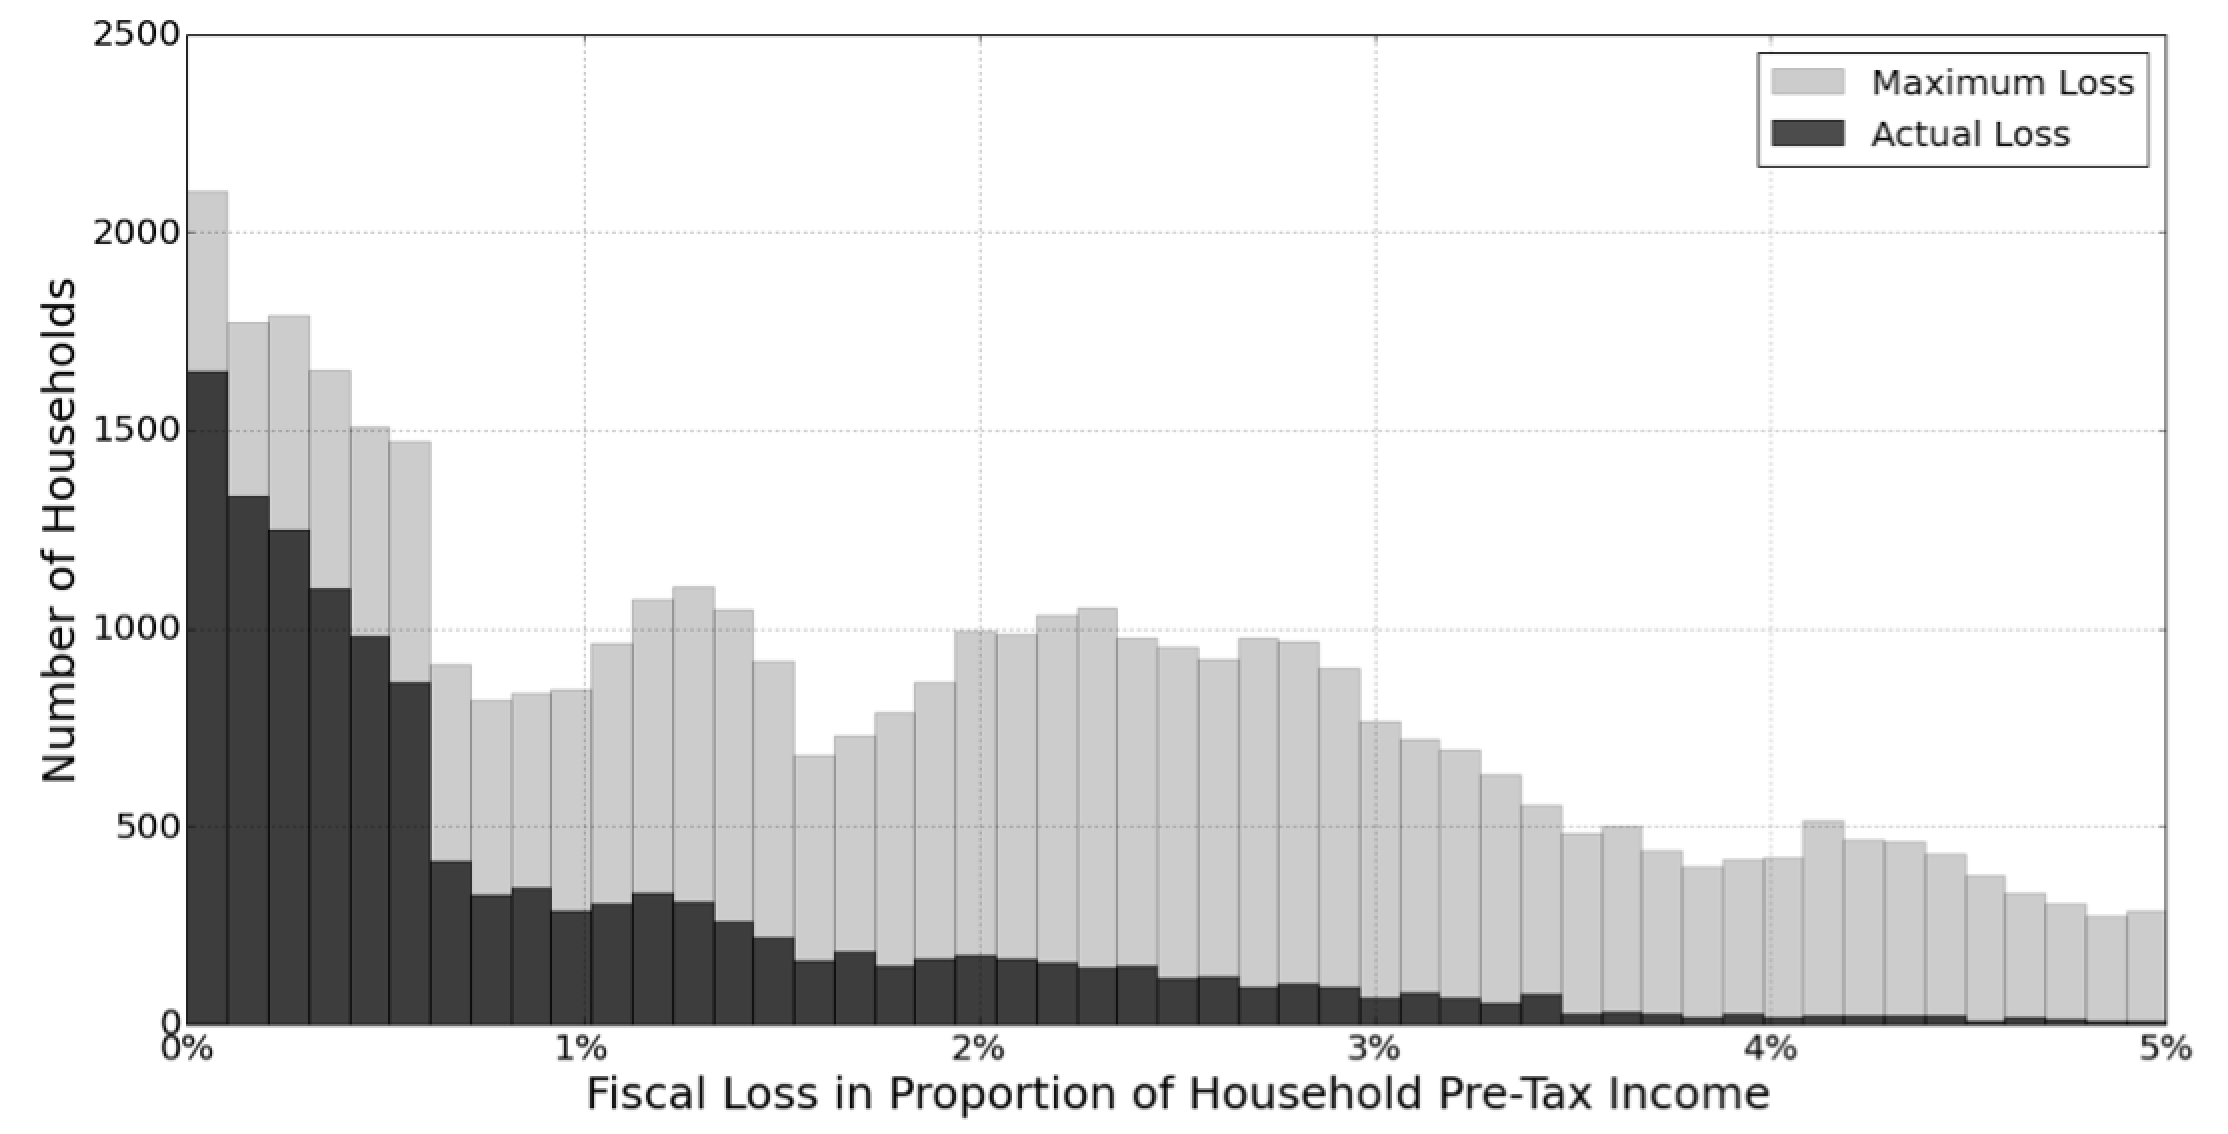
\includegraphics[width=1.1\textwidth]{figures/fiscal_loss_in_proportion.png}}%
    \label{fig:fiscal_loss_in_proportion}
    {\small
    Source: authors’ calculation using EDP data. Sample of cohabiting biological parents of children under 18. Selection for the graph excludes 11.3\% of couple who cannot optimize (the tax liability is the same whatever the allocation of children to one or the other parent).}
  \end{figure}


From fiscal data, we observe the actual choice made by cohabiting partners. Hence, for each household, we can determine whether it optimizes or not, i.e. whether it picks one of the child allocations that lead to the minimal tax liability. We can also compute actual losses, i.e. the gap in tax payment between the actual decision and the optimum. The distribution of actual losses is shown in dark bars in \autoref{fig:fiscal_loss_in_proportion}. We comment this results hereafter. Note at this stage that the distribution of actual losses follows somehow the non-linearity and discontinuities of the maximum loss profile, which are generated by various tax rules.

Table A.2 in the Appendix suggests a decomposition by demographic groups (number of children k). For each group, it shows how the number of optimal allocations is distributed, between polar cases (i.e. `only one allocation is optimal’ to `all the $k+1$ allocations are optimal’). Note that some of our results will be derived for the sub-group of couples for whom there is a margin of optimization. This group of potential optimizers (\textbf{PO}) excludes those located on the diagonal, i.e. those for whom all allocations are optimal (which represent 11.3\% of our selected sample: 8.9\% for whom tax liability is zero whatever children allocation and 2.4\% for whom all allocations lead to the same strictly positive income tax level). Results focusing on the PO will induce a slight bias against large families: as can be seen in Table A.2, the proportion of those who do not need to optimize increases with families of 3 and more (14.3\% for 3 children, 24.7\% for 4, 34.1\% for 5 and more). This pattern is simply explained by the fact that when a partner becomes non-taxable, because the assignment of one or two children has reduced enough the per-adult equivalent income of his/her tax unit, it is not necessary to allocate more children to him/her. We will also consider a sub-sub-group comprising those with only one optimal allocation among all possible allocations. The first column shows that they represent a large majority of cases for families with 3 children or less. Arguably, this selection of potential optimizers with a unique optimum (\textbf{POU}) will be biased towards smaller families.

\section{Conceptual Background and Potential Channels}\label{sec:section_4}

It is interesting to discuss the channels underlying potential tax return inefficiencies. Such a discussion will lead to suggestions about the informal checks that can be conducted in our empirical analysis. Not choosing the right child allocation – i.e. not minimizing tax liability – is clearly suboptimal and may be due to transaction costs (time to learn about the optimal allocation), cognitive biases (adoption of simple rules) or limited commitment problem within couples. We present in turn each of these channels.

The first pathway pertains to the question of whether a couple understands the tax rules and, then, undergo transaction costs to optimize. Arguably, the `family ratio’ system exists for decades and is very popular among French citizens as a large tax advantage for families with children. It was initially popularized as a contributor to the relatively high fertility rate in France compared to neighboring countries \citep{landais2004quotient}. Note that people are explicitly asked in their tax declaration how many dependent children they have and, in the case of cohabiting partners, are reminded that each child can be allocated only once (i.e. to only one of the two tax units). \footnote{
    Failing to do so is considered as tax fraud, and an official letter would prompt that couple to correct and jointly inform the authorities about who benefits from the child allocation.}
Then, the question is whether families can easily know what to do best. If we consider the case of couples with dependent children in 2013, they are young enough to be internet users and to be familiar with administrative information online, i.e. the tax authority website “impots.gouv.fr”.
In 2013, this website has been visited 103,1 million times, mainly to use the tax simulator (27.7 million simulations performed). The latter allows tax payers to simulate the tax amount they have to pay, asking them the same information as on tax forms (including child allocation) and processing it with exact tax rules. One may still argue that it can be cumbersome for cohabiting couples with a large number of children to simulate all the k+1 possible allocations – and we expect more inefficiency in this case – but certainly not for small families. In any case, we cannot rule out that transaction costs of that sort can explain sub-optimal decisions in some households, especially if the gains from searching the optimum are perceived as being rather small compared to the opportunity cost (of time) of doing so. In what follow, we will test whether inefficiency is correlated with family size or proxies for cognitive skills (like holding a higher degree).
More likely, sources of error related to cognitive biases may be due to specific heuristics applied in the case of tax filling. It is possible that people do not take an all-inclusive view of their finances  \citep{thaler1999mental}), so that mental accounting and `focusing illusion’ biases may offer an explanation for apparently irrational behavior. People may decide complex matters like tax by responding to the most salient or obvious aspect of a choice set or decision problem \citep{chetty2009salience,mccaffery2004framing}.  Fairness considerations also matter and may conflict with efficiency when thinking about tax design \citep{mccaffery2003heuristics}. In our context, the idea that both partners should benefit from the tax relief provided by children may prevail over a precise calculation of the optimal allocation. For instance, they may exert some sense of fairness attached to `equal split’, for those with 2 or 4 children – a bias that we can easily check in our empirical application. 

\medskip

This particular setting is more than an individual cognitive bias: it is a coordination problem where two partners are potentially unable to go beyond symbolic aspects. It may also be the case that they do not redistribute resources efficiently, so that we face a classic problem of dynamic non-cooperative behavior \citep{chiappori2017static}. This third type of explanation is easily described: an efficient decision would involve an optimal allocation of children to tax units coupled with a side-payment from the partner who benefits the most from child tax relief to the other partner. This may not happen because of heuristics and symbolic reasons, as emphasized above, or due to a lack of binding agreement between partners regarding the possibility to make these compensating transfers. Assume spouse m earns more than spouse f and try to convince her to associate all the children to his tax unit by promising to transfer some of the optimization gains. For instance, assume that partner m’s (f’s) pre-tax income is 200 (100) and his (her) tax liability is 100 (10) due to progressivity. He obtains a larger reduction (16) than her (10) if children are attached to his tax unit (rather than hers). In the former case, he transfers half of the gain, while in the latter, she makes no transfer (she’s already poorer). This is summarized as:

  \begin{table}[H]
    \makebox[\textwidth][c]{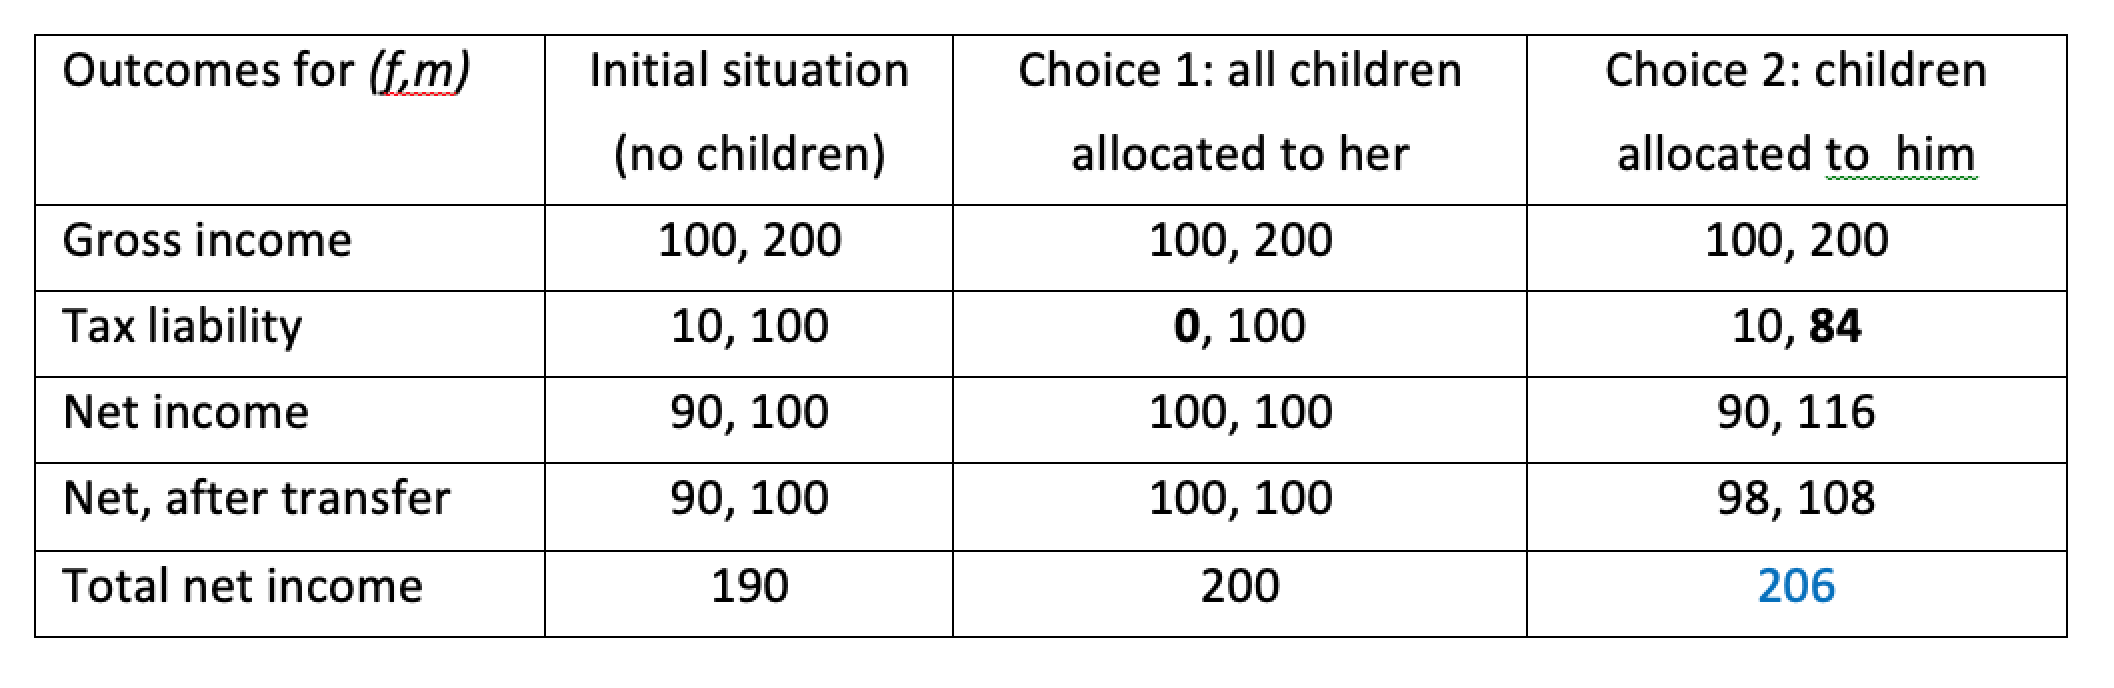
\includegraphics[width=1.1\textwidth]{figures/table_income_tax.png}}%
  \end{table}

The optimal choice is number 2 (children attached to him). She could accept it – even though the transfer does not make her as well off as with choice 1 – if she considers that they both win compared to the situation before the child was born (possibly taken as reference point) and win equally (+8 each). Conversely, she may ex ante refuse the arrangement 2, as she anticipates that redistribution will not be enough (he might actually promise more than half of the gain but agreements are not binding). She could then argue that choice 1 is neutral for him (compared to before the child arrived) and he might accept, especially if he already does not redistribute much of his own resources to her.\footnote{
    This type of inefficiency may materialize even more if there is asymmetrical information, which increases the limited commitment problem. Efficiency in collective models is based on the assumption of perfect information, yet recent evidence show that it is limited \citep{baland2017intra}. For instance, he may prefer choice 1 (she makes a gain of 10) rather than going into computation in search of an optimum, because these calculations would imply revealing exactly the large unbalance in net incomes between them and possibly lead to redistributive pressure. Another reason is that even in a situation with infinitely repeated interaction, the folk theorem shows that almost every allocation situated between a non-cooperative Nash outcome and the Pareto efficient outcome could be stable.  In other words, (infinitely) repeated interaction does not necessarily lead to efficient behavior (c.f. \citet{baland2017intra}).}

This example may characterize well the situation just after the arrival of the first child, which may be efficient or not, as described above. Renegotiation can take place the year after, at the next annual tax declaration.\footnote{
    The first year, a sequential game may also take place where one partner is taken by surprise, i.e. m fills his tax form first, leaving f facing this choice (see experimental evidence on “who holds the mouse”, in \citet{de2011individual}). Whatever the dynamic decision-making process, it is possible that a suboptimal allocation be chosen that reduces the tax paid by one spouse while the other is not fully compensated.}
Whether inefficiency is persistent or not can be checked over two years in our setting. It may last because of inertia in household decisions. Also, while the literature indicates that inefficiency especially concerns non-repeated, one-off decisions (for instance, location choices, as exemplified in Pollack et al., 2013), %TODO: cite 
lasting inefficiency for decisions that are regularly repeated, like tax filling, seems a stronger case of non-cooperation.\footnote{
    Tax payments are made in three installments in February, May, September (for 40\% of French taxpayers) or monthly (for 60\% of them). Early payments in the year are based on past-year information. The tax declaration (including child allocation) is made in May/June, leading to adjustment in payments (i.e. in the September installment or in the monthly installments following the tax declaration).}
Strong disagreements may results in separation, or less chances of more engagement (marriage), which is something we will test hereafter.


\medskip 
Finally, remark that several studies reject the efficiency of household decisions for the allocation of productive inputs, in the context of developing countries – for instance \citet{udry1996gender}, \citet{duflo2004intrahousehold} and \citet{apedo2017}.
 We can actually make an analogy to this literature if the process of allocating children to the man or the woman is a particular form of production decision, affecting the resources controlled by each partner, and requiring some cooperation if the couple wants to maximize total resources. Even if the household is efficient for consumption decisions, this previous, productive step may fail to provide overall efficiency.\footnote{
     Other forms of inefficiency involve imperfect risk sharing \citep{dercon2000sickness,robinson2012limited}, strategic appropriation of resources \citep{anderson2002economics}, lying and hiding \citep{ashraf2009spousal}, strategic use of violence \citep{bloch2002terror}. As investigated in \citet{baland2017intra}, potential explanations pertaining to the role of time and uncertainty, the lack of commitment, the role of irreversible decisions and asymmetric information between spouses, among other things that applied to both poor and rich countries. The literature also highlights under-contribution to public goods through the use of experimental games between spouses (Hoel, 2015).  Theoretically, a few papers try to restore some of the efficiency thanks to love or caring \citep{browning2009consumption, cherchye2015noncooperative}. Experimental evidence often points to inefficient decisions, see the recent survey of \citet{munro2018intra}.}
We now move to the empirical part in order to measure the rate of rejection of such a `productive efficiency’.
\section{Results}
\subsection{Main Results}
\paragraph{Inefficiency rates.}
The main results are provided in \autoref{tab:table_1}. We consider the whole selection of cohabiting couples with children under 18, the sub-group of PO and the sub-sub group of POU. In each of these three nested samples, we report the distribution of cohabiting couples by family size (column 1), the number of non-optimizers (column 2) and their proportion (column 3). We find a non-negligible rate of inefficiency: there are 24.8\% of non-optimizers overall, 28\% among those who can optimize (PO) and 29.1\% among those with only one optimization possibility (POU). The average loss among non-optimizers is around 320 EUR, which corresponds to 0.9\% of pre-tax income on average (or 14.9\% of average tax payment). Since these overall figures may hide a tiny bias against large families, as described above, we also comment on the inefficiency rate by family type. We see that for small families, the proportion of non-optimizers (e.g. 28.4\% in couples with two children) increase mechanically when focusing on PO (31.5\%) and increases still when looking at POU (34\%). 


\medskip
The rate of non-optimization for POU literately explodes in larger families but these are not so relevant because moving to POU considerably reduces sample size in their case. An interesting pattern, both for the baseline selection or the sub-groups PO and POU, is the fact that inefficiency rates are larger for families with an even number of children (2 and 4). A possibly explanation is the use of simple allocation rules like ‘equal split’ (we come back to this point in our interpretations below).


\medskip
These results can be mitigated if we look at large income losses. \autoref{tab:table_1} reports the number (column 4) and proportion (column 5) of couples who commit large optimization errors (i.e. large inefficiencies), defined as income losses larger than 1\%. This proportion is around a third of all inefficiencies, i.e. 8.2\% of cohabiting couples, and increases naturally when looking at PO (9.3\%) and POU (9.5\%). We find the same pattern as above: (large) inefficiency rates are bigger for families with 2 and 4 children. 




 \medskip

  \begin{table}[H]
  \caption{Rate of Non-Optimization (and Large Non-Optimization) by Demographic Groups}
  \label{tab:table_1}
    \makebox[\textwidth][c]{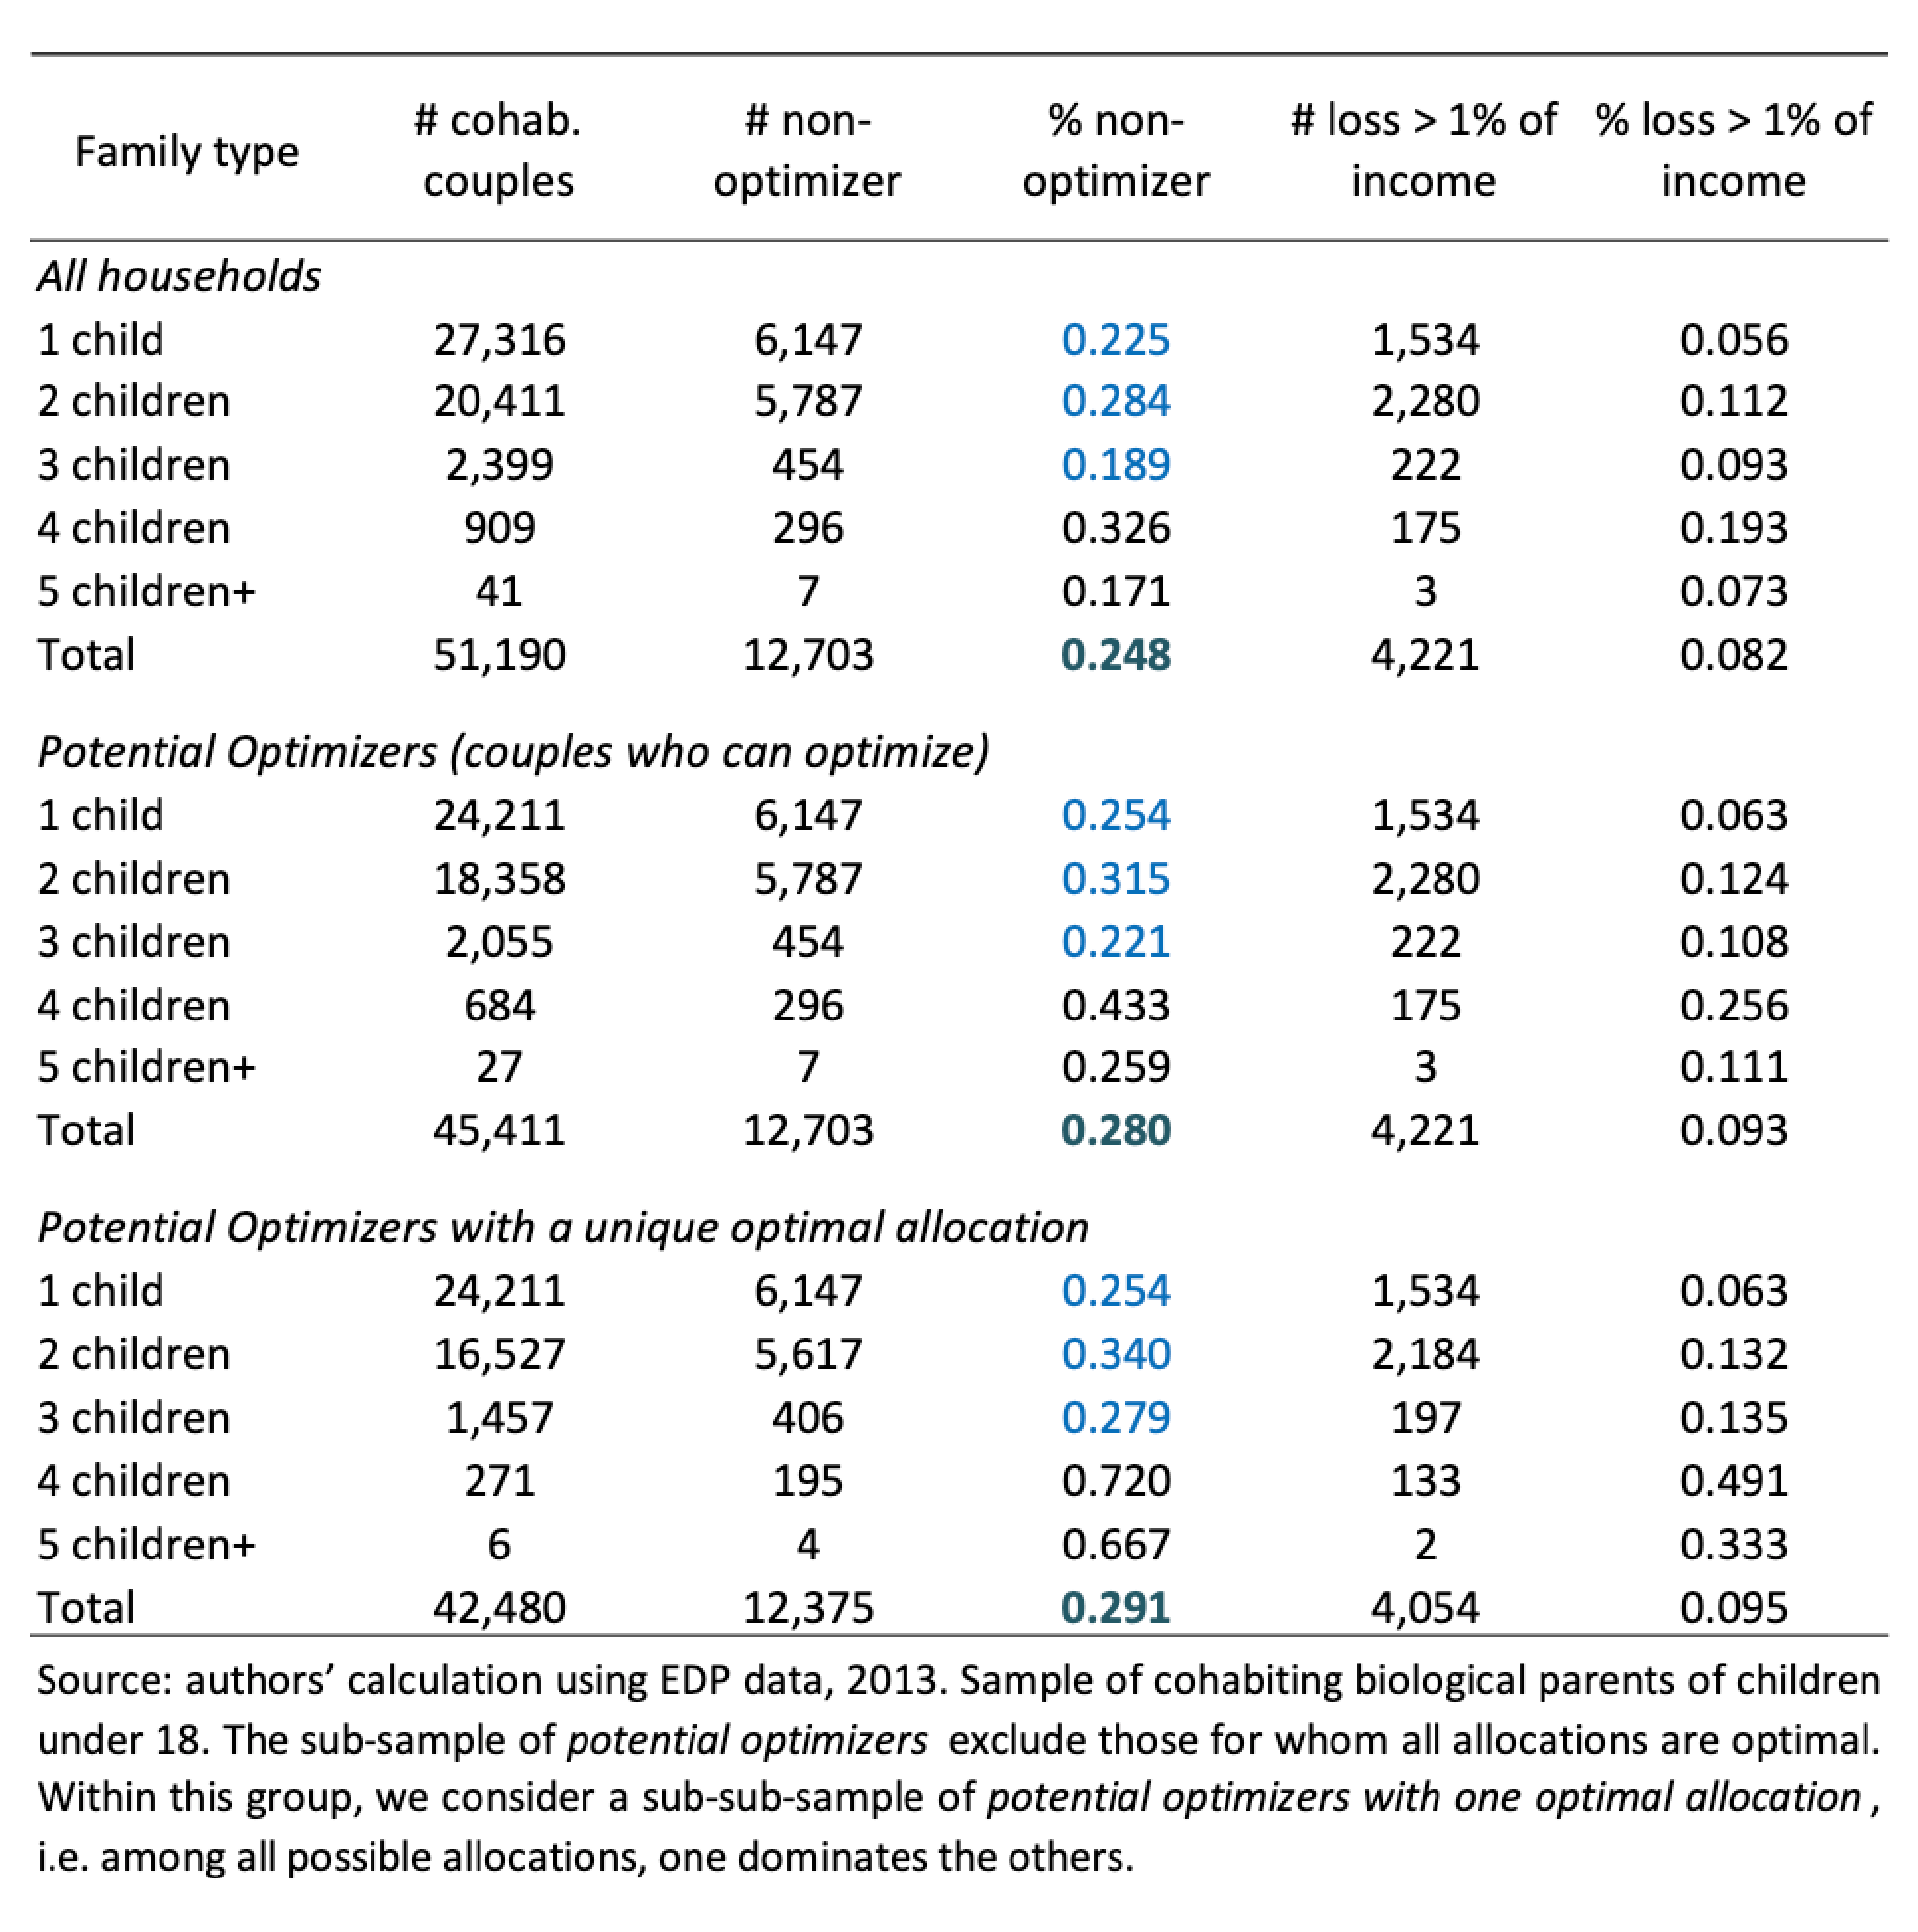
\includegraphics[width=1.1\textwidth]{figures/table_1.png}}%
  \end{table}

The proportion of actual losses can be compared to the distribution of maximal losses. The distribution of actual losses is represented by the dark bars in \autoref{fig:fiscal_loss_in_proportion}. It shows a high mass of error at lower levels, between 0.1 and 0.5\% of income. The density of errors then decreases regularly from 0.6\% to around 5\% of income. Additional statistics are as follows. We have seen that 70\% of the PO (cohabiting couples who can optimize) have their worst allocation exceeding 1\% of income. In fact, 13\% of the PO choose this allocation (9.3\% of the baseline sample), i.e. commit what we have defined as a large inefficiency.




  \begin{table}[H]
  \caption{Distribution of Optimizers by Demographic Groups and Allocation Type}
  \label{tab:table_2}
    \makebox[\textwidth][c]{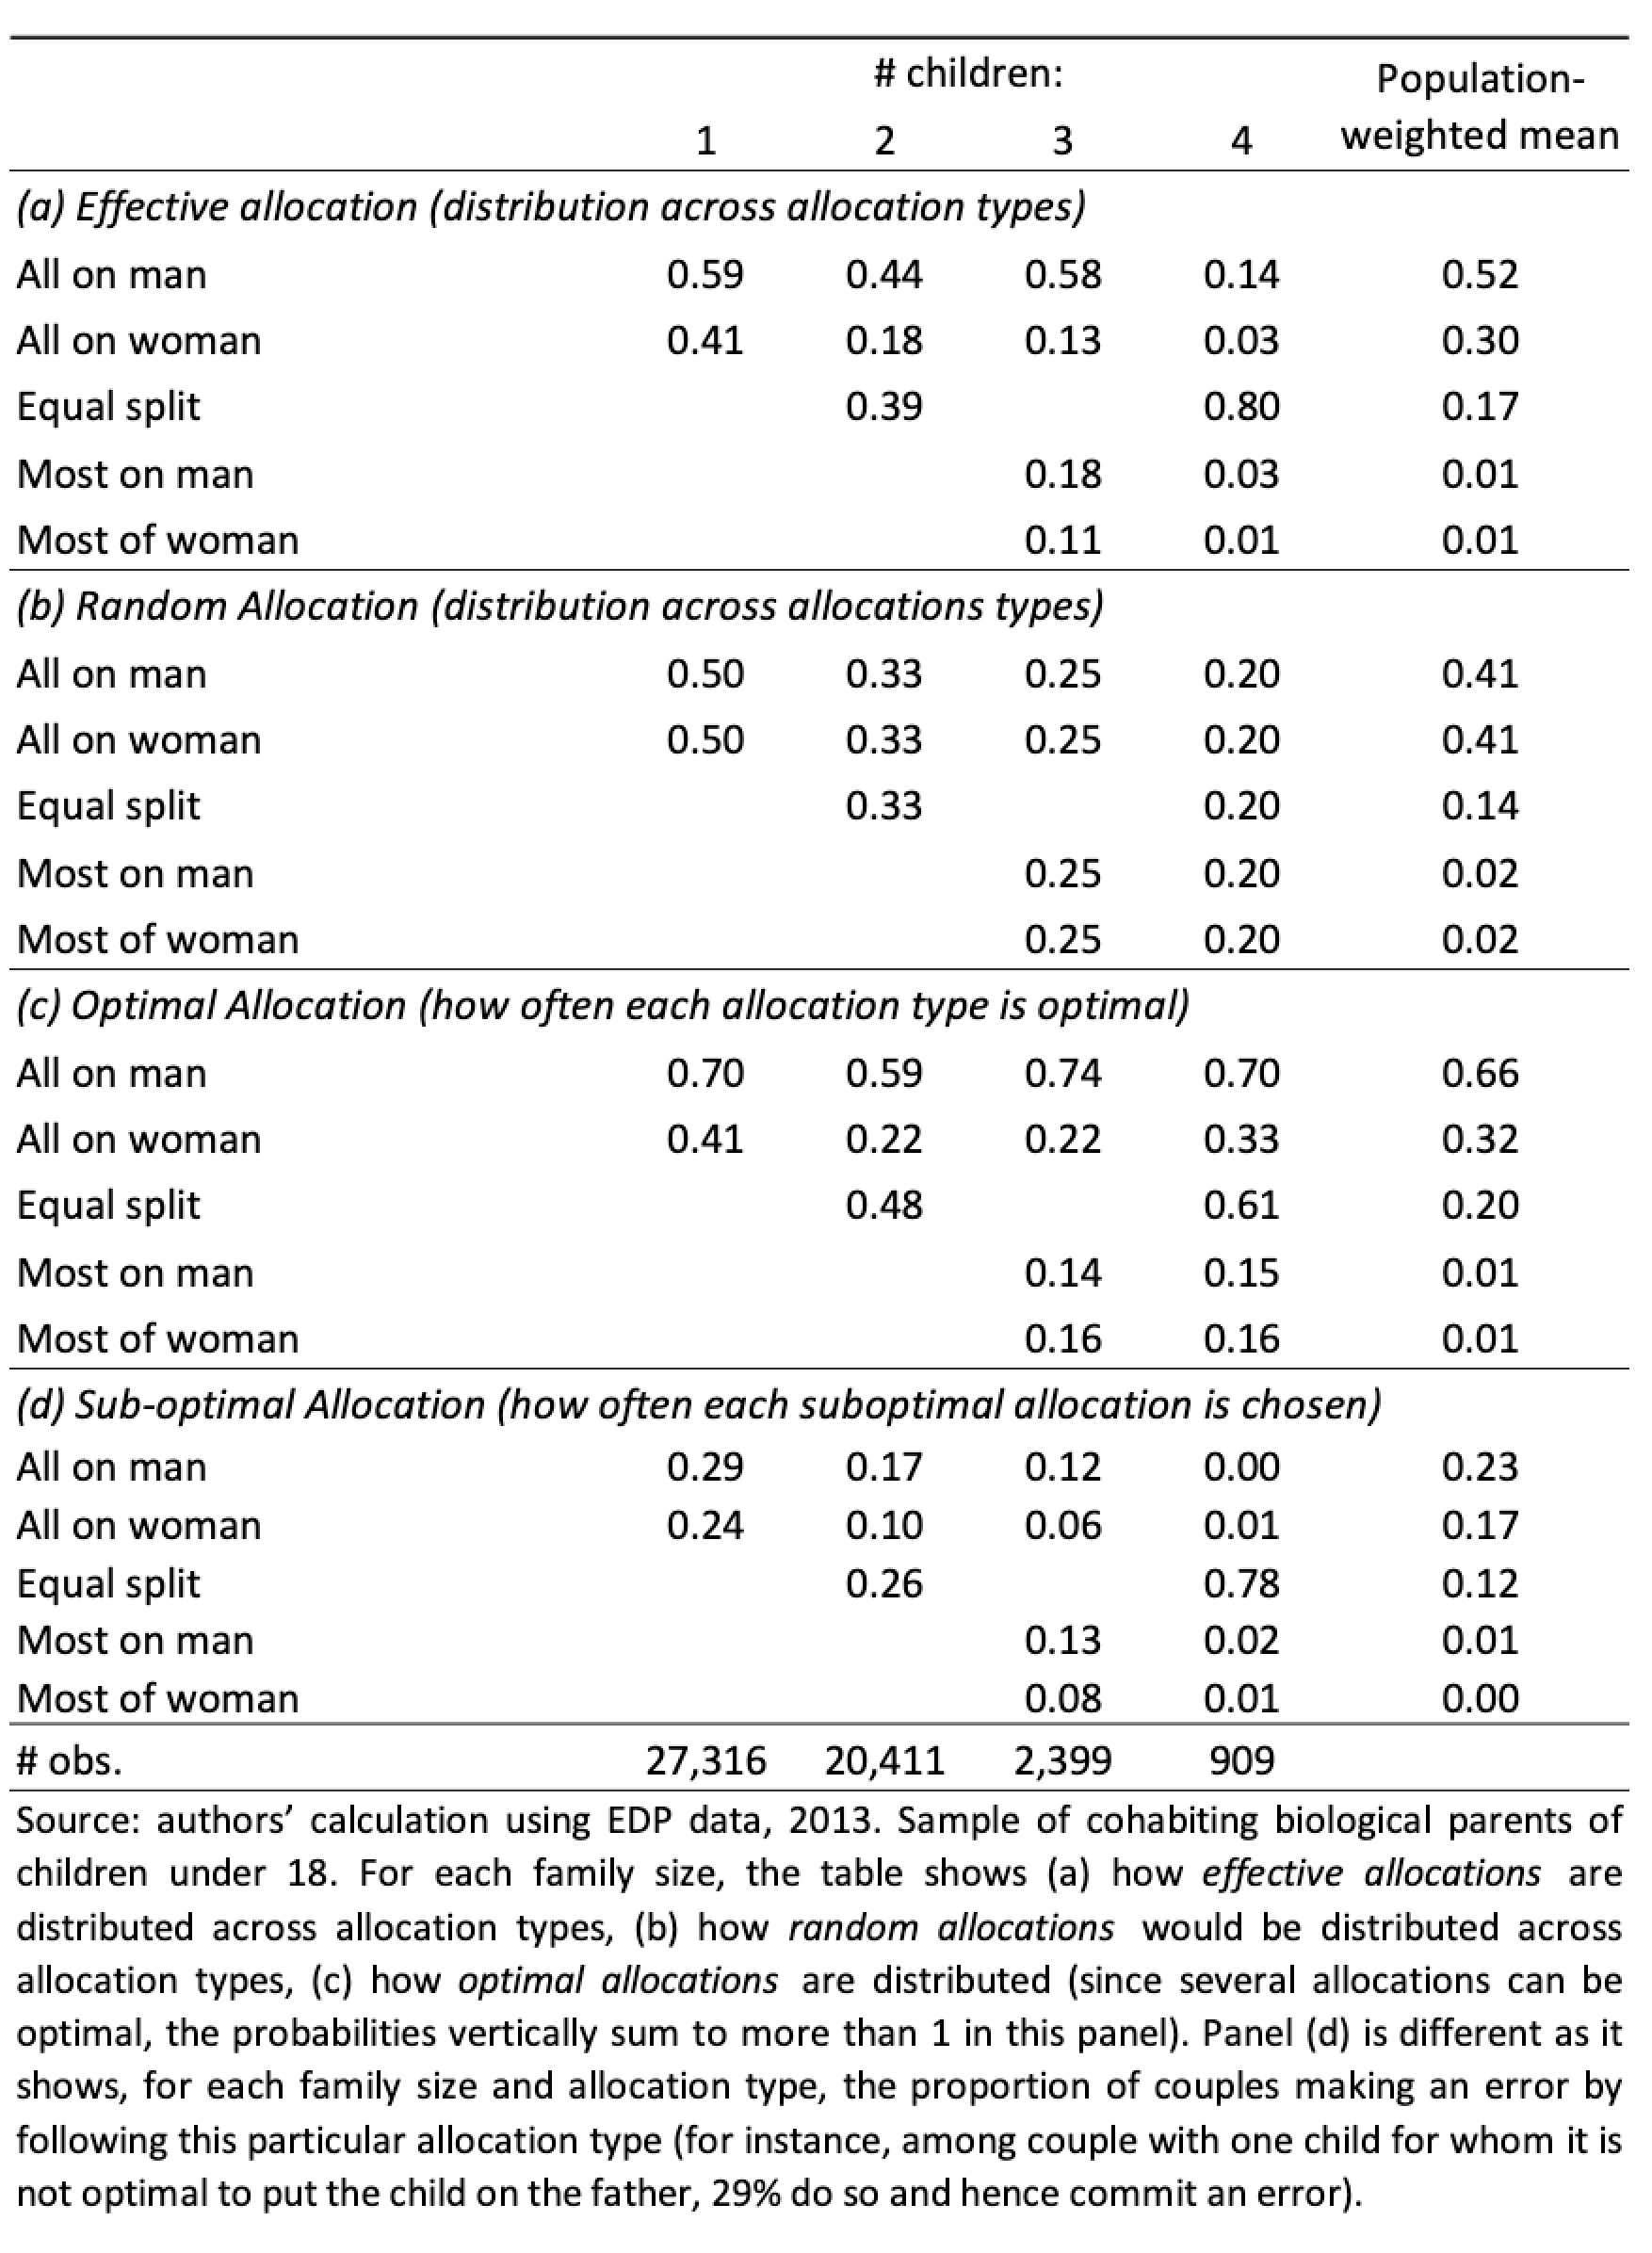
\includegraphics[width=1.1\textwidth]{figures/table_2.png}}%
  \end{table}

\paragraph{Patterns of inefficiency. }
Beyond mean rates of inefficiency, we suggest more analysis in \autoref{tab:table_2} (we focus on families of 1-4 children since larger families are very few). Panel (a) shows the distribution of actual allocations, by family size and type of chosen allocation (“all children on father”, “equal split”, etc.). Panel (b) shows the distribution in case of random allocations. Chi-squared tests of (a) versus (b) indicate that effective allocations deviate significantly form random allocations (all p-values are 0 for all family sizes). For instance, in couples with one child, 59\% of them put the child on the father’s tax return, which is significantly different from a random allocation of 50\% in this case. 




\medskip
For each allocation type and demographic group, panel (c) reports how frequently this allocation is optimal. These frequencies vertically sum up to more than 1 because several allocation can be simultaneously optimal. For this reason, the panel (c) is not directly comparable to (a) and (b), but gives useful indications. For instance, in couples with one child, it is more often optimal to put the child on the father’s tax unit (optimal for 70\% of the couples) than on the mother’s (41\%). Importantly, actual allocations tend to deviate in this direction compared to the random allocation, as seen above. For families with four children, our conjecture of a bias associated to the simple ‘equal split’ rule seems to apply: this equal allocation is chosen in a majority of cases (80\%) while it is not so often optimal (61\%).


\medskip
Other biases may be at work but not visible in these results. For instance, putting all the children on the father, as main earner, may be another heuristics. Yet this choice may effectively be often optimal at the same time. In order to detect the influence of ‘simple rules’, we extract information on the frequency of typical errors in panel (d). For families with one child, the first row shows that among all the couples for whom it is non-optimal to put the child on the father, 29\% choose to do so. This type of error seems also present in families of two and three. In couples with four children (and to a lesser extent with two), we observe very suggestive evidence of the `equal split’ bias. As discussed, this simple and apparently fair rule may not be simply a form of heuristic but also a sign of cooperation failure between partners.


\medskip
\paragraph{Profile of the non-optimizers. }

To carry on this descriptive analysis of tax sub-optimization, we suggest a simple regression of the non-optimization status on basic characteristics. Results are reported in \autoref{tab:table_3}. The first two columns focus on our baseline sample (we have obtained very similar results using PO and POU samples, and we simply provide specific comments below in case of significant differences). Consistently with the risk of choosing `equal split’ in the case of an even number of children (as documented in \autoref{tab:table_1}), families with two and four children have a significantly larger probability of making an optimization error overall, or a large error in particular, relatively to the omitted group (i.e. those with one child). The age of the older child seems to be a good marker of a couple’s duration and, hence, its chances of reaching efficiency through cooperation and coordination. It also corresponds to the time during which the cohabiting couple faces an optimization problem in terms of child allocation, hence the time to learn about tax rules or the possibility to simulate tax liabilities under different allocation scenarios. Controlling for parents’ age and the number of children, the older child’s age is indeed correlated negatively and significantly with the probability of missing the optimal allocation. Maybe counter-intuitively given the previous argument, older couples are more likely to be inefficient overall (but not to commit large errors). The chances of optimization error increase with the couple’s income, essentially because low-income couples correspond to more salient situations (the wife is more frequently out of the labor market in poorer households while her partner is tax liable only if the children are not allocated to him). The probability of large errors, on the other hand, is decreasing with income, which may be related to the fact that rich families tend to more systematically optimize their finance. Another source of tax optimization is, for cohabiting couples, the option to enter a civil union. As said, it allows them to benefit from the tax treatment of married couples without the need to get married. We find that those who would gain much to do so, and do not, are also more likely to sub-optimize child allocation.


  \begin{table}[H]
  \caption{Profile of the Non-Optimizers}
  \label{tab:table_3}
    \makebox[\textwidth][c]{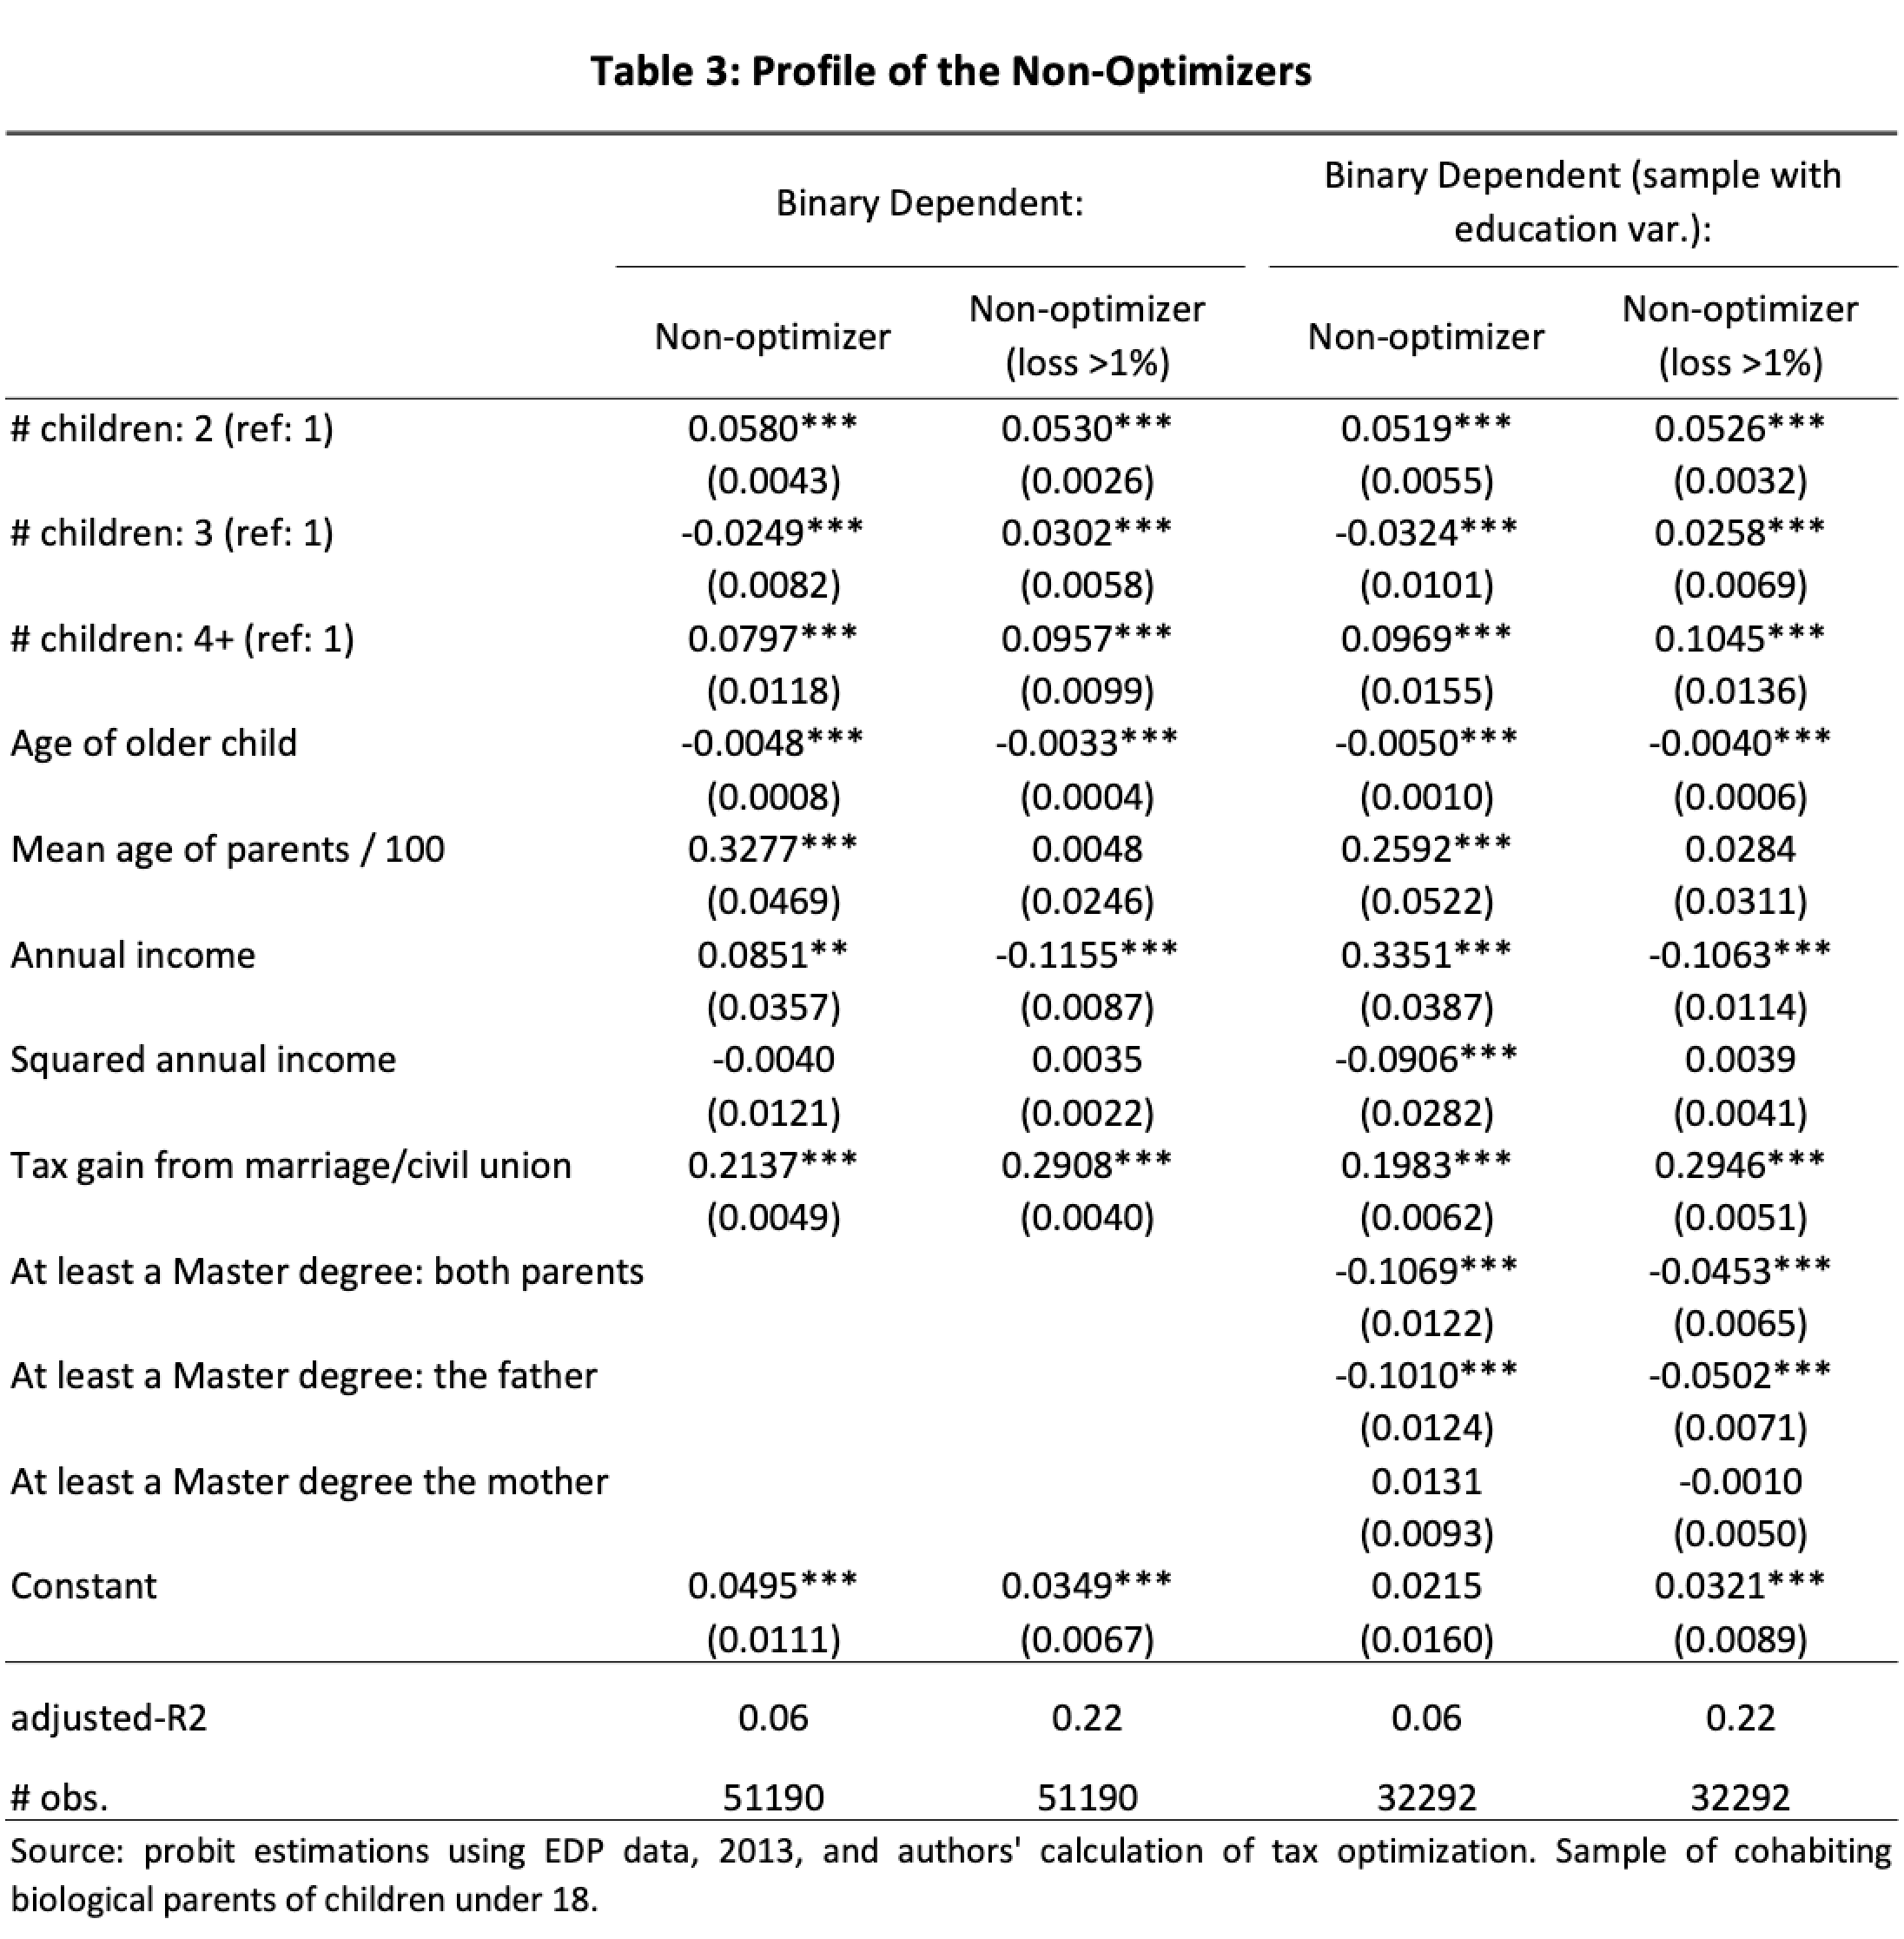
\includegraphics[width=1.1\textwidth]{figures/table_3.png}}%
  \end{table}

The last two columns show the result of regressions conducted on the smaller sample containing education variables. For the common set of covariates, these results are very comparable to those on the whole sample, despite the aforementioned bias towards small areas. In order to check for cognitive skills, we add education variables. It turns out that in couples where both parents hold a master degree or a PhD (or when the father holds these higher degrees), optimization errors are less frequent, which may relate to the ability of more educated couples to understand tax rules and optimize. \footnote{
    Alternative estimations including a dummy for locality size – hence to account for the sampling bias in this smaller sample – give similar results.
} 


\medskip
A detailed breakdown of the causes of inefficiency is beyond the scope of the present paper and would probably require experimental evidence. Nonetheless, we can provide suggestive evidence about potential cognitive biases (sub-section 5.2) and non-cooperative behavior (sub-section 5.3) in what follows, drawing from the discussion of \autoref{sec:section_4}.

\subsection{Transition patterns, Learning and Inertia. }
We first present the transition patterns in terms of tax optimization behavior. We characterize transitions between 2013 and 2014 using panel information for those who remain cohabitants and experience, in both years, the problem of allocating children to two tax units.\footnote{In other words, those who get married or enter a civil union in 2014 are not in the picture. If these new unions are seen as a form of tax optimization, and a reflection of cooperative behavior, then the characterization that follows concerns a slightly different group from our initial 2013 sample, i.e. a group by definition less likely to coordinate well.
}
To clarify the analysis, we focus on couples with a fixed number of children over the two years, which have only one optimal allocation in both years (this optimal allocation may change). The subgroup with these characteristics represents 24,514 households, i.e. a large enough group – even if more specific than the baseline – to derive interesting observations. 


\medskip
Transitions are reported in \autoref{tab:table_4}. We first distinguish optimizers and non-optimizers in 2013, which are in very similar proportions as in baseline results for POU (c.f. \autoref{tab:table_1}), namely 71\% and 29\%. The second column splits these groups according to whether the (unique) optimal allocation has changed over time or not. Reasons for a possible change comprise a change in earnings (due to events such as job loss, wage rise, retirement, etc.) and small tax reforms that have taken place between the two years. \footnote{
    These reforms include change in tax bands (i.e. an uprating of 0.8\%, which is lower than wage inflation and hence may generate a little bit of `bracket creep’), a change in the maximum tax relief due to the family ratio system (namely a decrease of p from 2000 to 1,500 EUR per half fiscal shares) and a small change in the tax credit mechanism that benefits to couples with low tax liability (décote fiscale).}
 We observe that only a minority of couples have experienced changes that are large enough to affect the optimal choice. 



  \begin{table}[H]
  \caption{Transitions for Demographically Stable Couples\\ 
(Only One Allocation is Optimal each Year)
}
  \label{tab:table_4}
    \makebox[\textwidth][c]{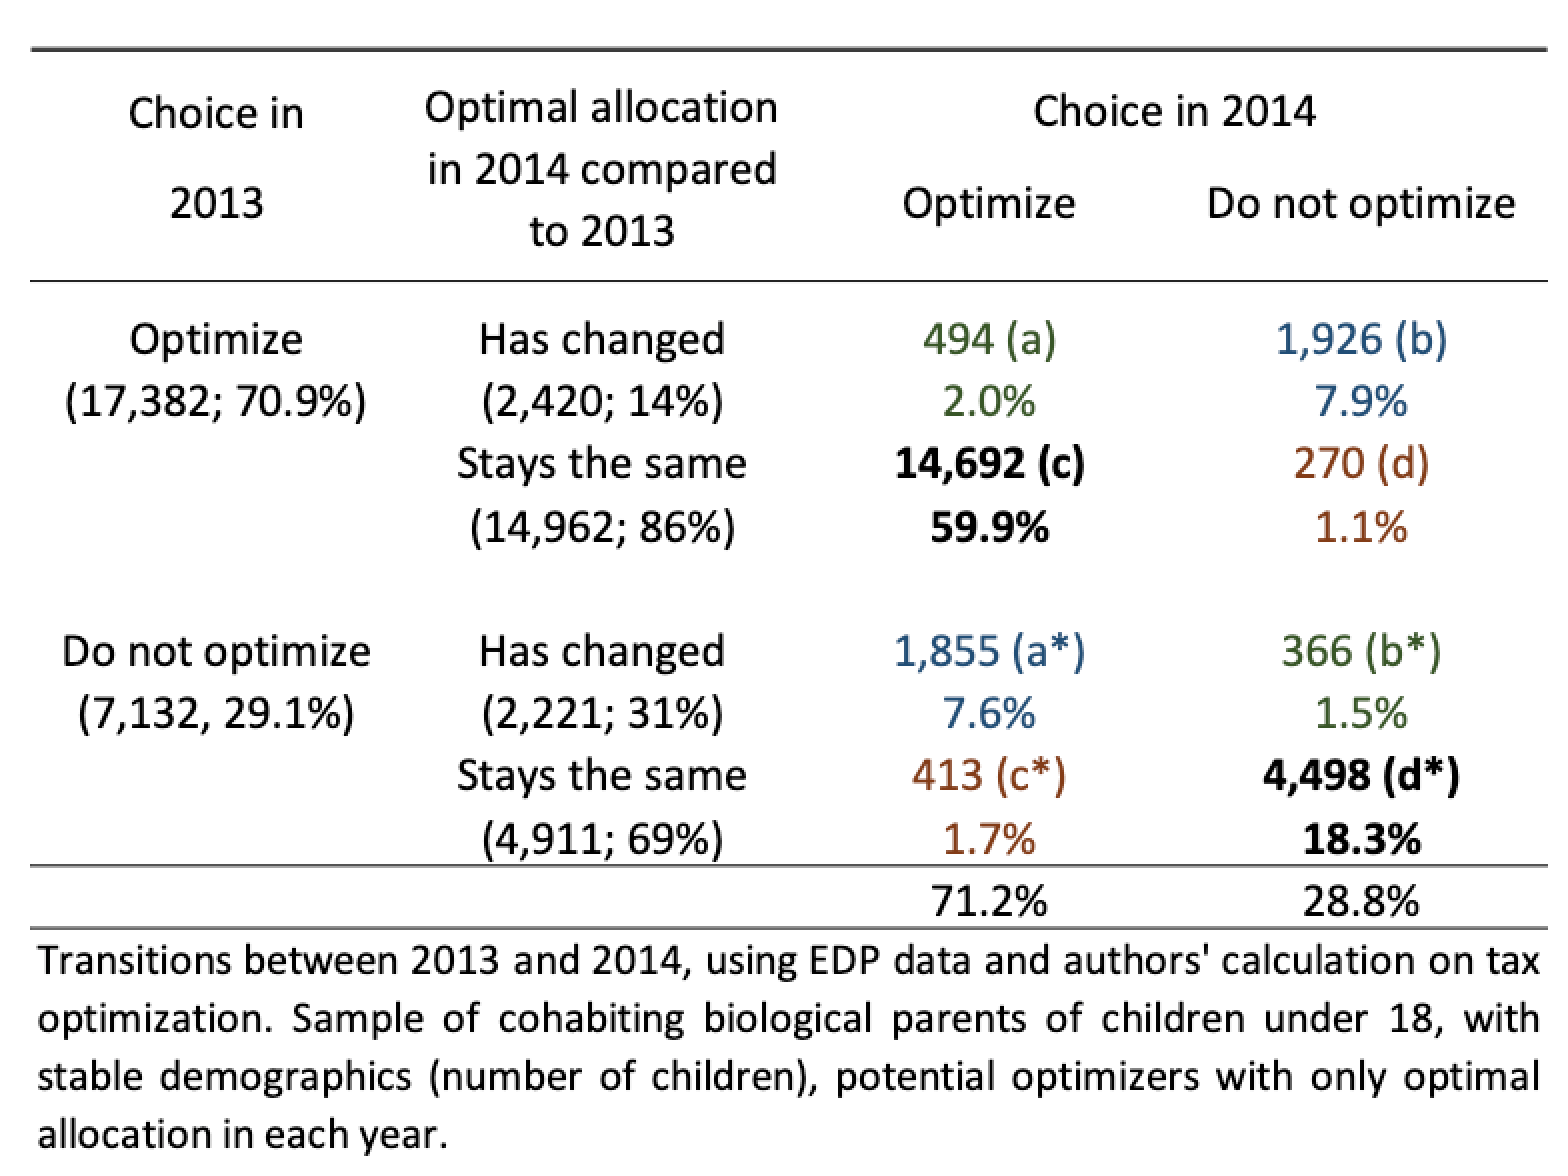
\includegraphics[width=1.1\textwidth]{figures/table_4.png}}%
  \end{table}

Then, we study the optimizing behavior in 2014. The proportion of non-optimizers is similar as in 2013 (28.8\%). The different cells in the last two columns suggest a breakdown across the different situations (all frequencies sum up to 1). The largest groups are composed of couples whose unique optimal allocation has not changed over time and who remain optimizers (group c, 59.9\%) or non-optimizers (group d*, 18.3\%). By definition, all couples in group c make the same decision upon child allocation as in the previous year. In group d*, 99\% have also not changed their decision, so that inertia may play a role, in addition to the cognitive biases or non-cooperative behavior that explained non-optimization in 2013 and may persistently explain it in 2014. Non-optimizers represent 23.4\% of the group c+d* characterized by stable optimal and actual allocations: this intertemporal rate of inefficiency shows only a small improvement compared to the static rate for 2013 (29\%). 


\medskip
Two other cells with constant optimal allocations concern those who change their child allocation and, hence, for whom we expect a majority of learners (it may be learning on how to optimize tax or how to improve cooperation/coordination in their couple’s decisions overall). This indeed the case, as the proportion of those switching to optimization (group c*) is much larger than those moving opposite direction (group d). 


\medskip
There is a much larger group with these patterns of transitions – learning or deteriorating – in the case of a change in the optimal allocation (groups a* and b). In this case, the numbers of transitions each way are relatively similar because both groups a* and b are `involuntary movers’: both are actually composed at around 98\% of couples who did not update their child allocation between the two years while the optimal allocation has changed. Group a* who seems to improve in 2014 may have just experienced lucky inertia or may have been close enough to the right allocation in 2013 while it now fully optimizes in 2014. Additional calculations indeed show that the average fiscal loss of group a* in 2013 was much smaller than the average loss.\footnote{Similarly, group b seems to deteriorate but may have experienced unlucky inertia or switched from optimization in 2013 to a slight sub-optimization in 2014. Additional calculations show that the fiscal losses of group b in 2014 was also a bit smaller than average. Note also that those who face a new optimum and need to make a change to reach it (a and b*) are the counterparts of the two main groups (c and d*) but cannot benefit from lucky inertia. The former (a) are optimizers who adjust their choice to the new optimum. The latter (b*) constantly opt for a suboptimal allocation: among them, 75\% are subject to inertia but not a lucky one (their choice is suboptimal in both years).}

\section{Noncooperation}

We finally check whether the lack of cooperation possibly revealed by tax inefficiency is associated with specific time trends in marital status. As discussed in section 4, it is expected that non- cooperative couples tend to marry less and to separate more. We start from our initial sample of potential optimizers in 2013 (45,411 observations) and check their marital transition between 2013 and 2014, i.e. whether each couple has stayed unmarried, got married, got in a civil union or separated. Since only large non-optimization losses may reveal non-cooperative behavior, we focus on losses above 1\% of income (the basic non-optimization definition does not yield results that are as compelling as what follows).


\medskip
We find that the rate of new marriage in 2014 among those who optimized in 2013 is 10\% larger than among those who did not optimize, while the rate of separation is 32\% lower. To go beyond basic statistics, and to control for household characteristics that could possibly affect these trends, we estimate a multinomial logit with the four categories of transitions in marital status between 2013 and 2014 (the omitted category is status quo). We control for the basic covariates previously used in the profile of non-optimizers. Remember that we conduct these estimations on the PO sample but sensitivity analyses are discussed hereafter.


\medskip
Results in \autoref{tab:table_5} are striking, even if merely suggestive and descriptive: being non-optimizer in 2013 is associated with significantly higher chances of separation in 2014 and significantly lower probabilities of marriage or civil union. The table reports marginal effects: the change in marital status probability corresponds to 0.6 percentage points in the case of separation, -0.9 points for marriage and -0.6 points for entering civil union. Other variables are interesting. Larger families tend to get married more than those with one child but not to get a civil union. Couples’ duration (as proxied by the age of the older child) is associated with higher chances of separation and lower chances of getting in a civil union. Richer couples seem more stable as they tend to separate less and marry/unionize more. The existence of a fiscal gain from marriage/civil union has an effect on all transitions other than the status quo, but it is especially large for the chances of getting a civil union and, to a lesser extent, of getting married.




\medskip
Sensitivity checks are reported in \autoref{tab:A3} in the Appendix. We alternatively use the baseline selection, the subsample of PO (i.e. the baseline estimates from Table 5), the nested sample of POU: all three samples yield similar results. Then we focus on the smaller sample containing education variables, which we now control for. Estimates lead to the very same conclusions. The last row shows the regression where we vary the non-optimization definition and lower the loss level at 0.5\%, i.e. non-optimizers are those who loss more than 0.5\% of annual income. The correlation with marital transitions is arguably smaller (and become insignificant in the case of marriage) but points to the same type of interpretations.


  \begin{table}[H]
  \caption{Correlation between Change in Marital Status in 2014 and Non-optimization in 2013 )
}
  \label{tab:table_5}
    \makebox[\textwidth][c]{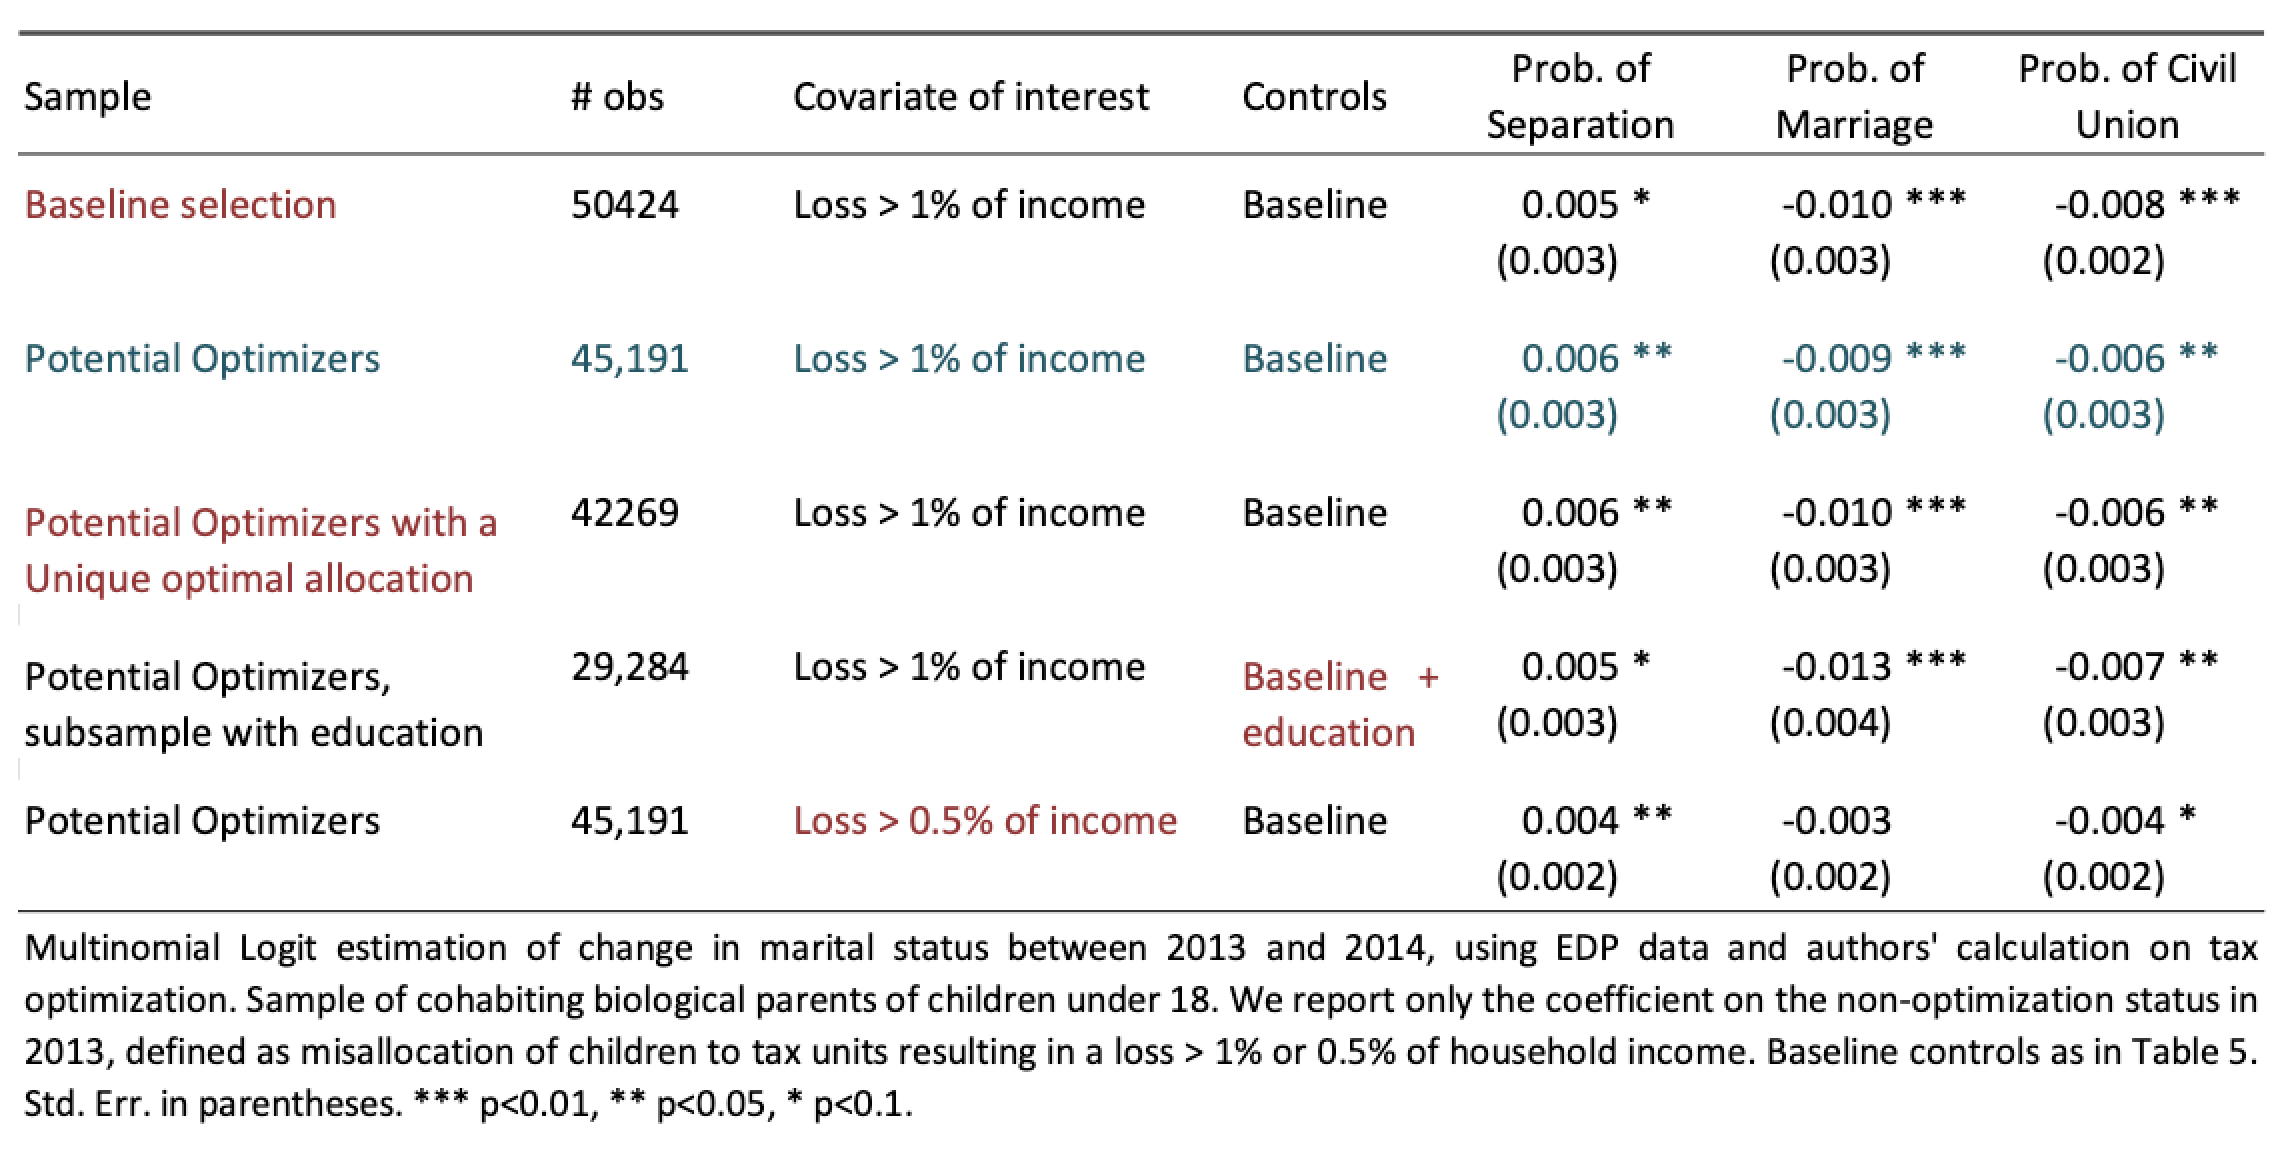
\includegraphics[width=1.1\textwidth]{figures/table_5.png}}%
  \end{table}

\section{Conclusion}
We suggest a direct measure of cohabiting couples’ inefficiency for a repeated decision that affect the budget constraint, namely tax optimization via the optimal allocation of children to tax units. We find a non-negligible fraction of non-optimizers in both years (29.1\% in 2013 and 28.8\% in 2014). We find traces of heuristics (like equal split, when the number of children is even, or putting all children on the main earner). The portrait of non-optimizers shows that durable couples tend to allocate children more optimally while those who sub-optimize in other domain (e.g. do not enter a civil union while they would gain much from it) tend to misallocate. There is little learning and much inertia: 81.8\% of the couples stay in the same optimization status over both years (61.9\% optimizers, 19.8\% non-optimizers). When the optimum is stable, persistence is even higher, with 96.6\% of stable statuses (73.9\% optimizers, 22.6\% non-optimizers) – in the remaining 3.7\%, a majority (60\%) seems to learn, i.e. start to optimize. When the optimum changes, the transition pattern reveals a majority of new situations of optimizations (40\%) or of non-optimization (41.5\%), which again reflects inertia because most couples do not change their choice and hence get lucky or lose the optimum (in both cases, they gravitate close to the Pareto frontier as fiscal loss is minimum). Finally, we find that large inefficiencies in 2013 are associated with higher moves towards separation (and lower transitions towards marriage or civil union) the following year. This is suggestive evidence of the role of non-cooperation as a primary mechanism for tax inefficiency.

Further work should look at the dynamic over several years in order to check if inefficient couples eventually improve upon learning or cooperation and eventually achieve efficiency. To decipher the mechanisms at work in the group of inefficient couples, new research could suggest experiments with real couples or with pairs of individuals, playing tasks that mimic real-world decisions regarding tax filling and a (productive) allocation problem (see the lab-in-the-field experiment of \citet{apedo2017}
, regarding productive decisions upon resource allocation in the context of a poor country).


\newpage
\addcontentsline{toc}{section}{References}
\bibliography{cohabiting_couples}
%%%%%%%%%%%%%%%%%%%%%%%%%%%%%%%%%%%%%%%%%%%%%%%%%%%%%%%%%%%%%%%%%%%%%%%%%%%%%%%%%%%%%%%%%%%%%%%%%%%%%%%%%%%%%%
\begin{subappendices}
\section{Descriptive Statistics}
  \begin{table}[H]
    \caption{Descriptive Statistics}
    \makebox[\textwidth][c]{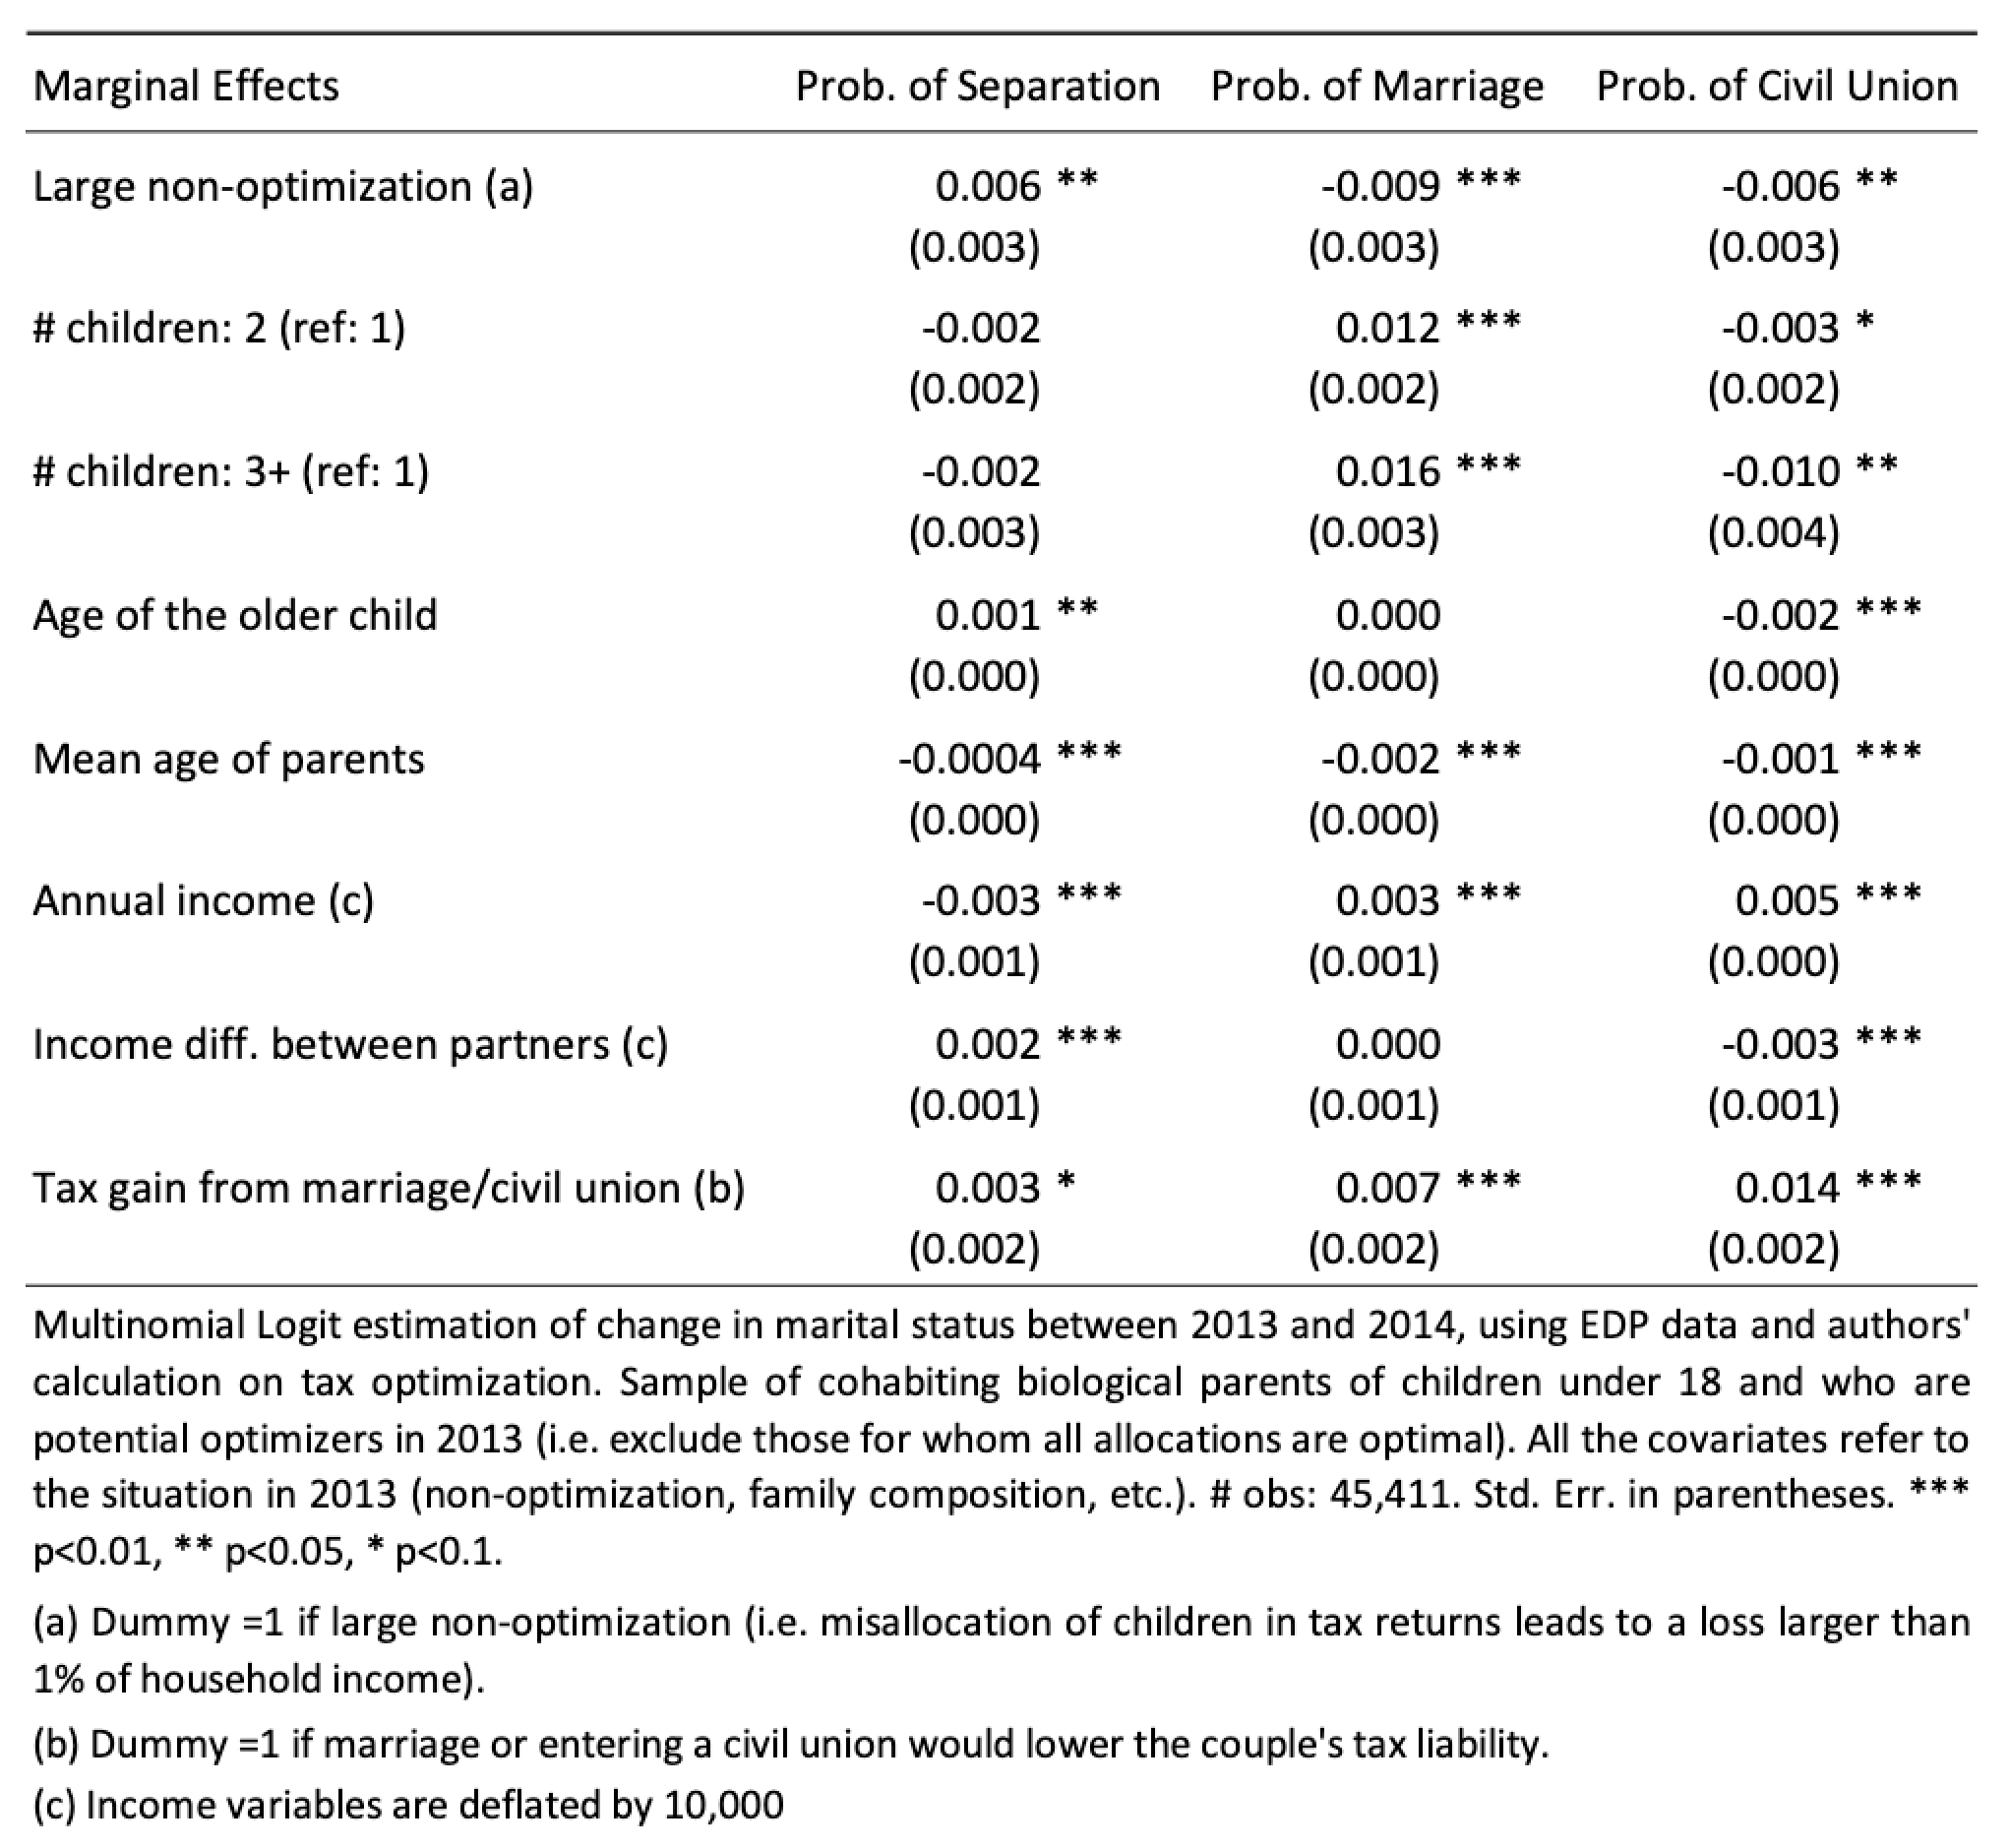
\includegraphics[width=1.1\textwidth]{figures/table_A_1.png}}%
    \label{tab:A1}

  \end{table}
  \section{Distribution of Optimal Allocations by Family Size}
  \begin{table}[H]
    \caption{Distribution of Optimal Allocations by Family Size}
    \makebox[\textwidth][c]{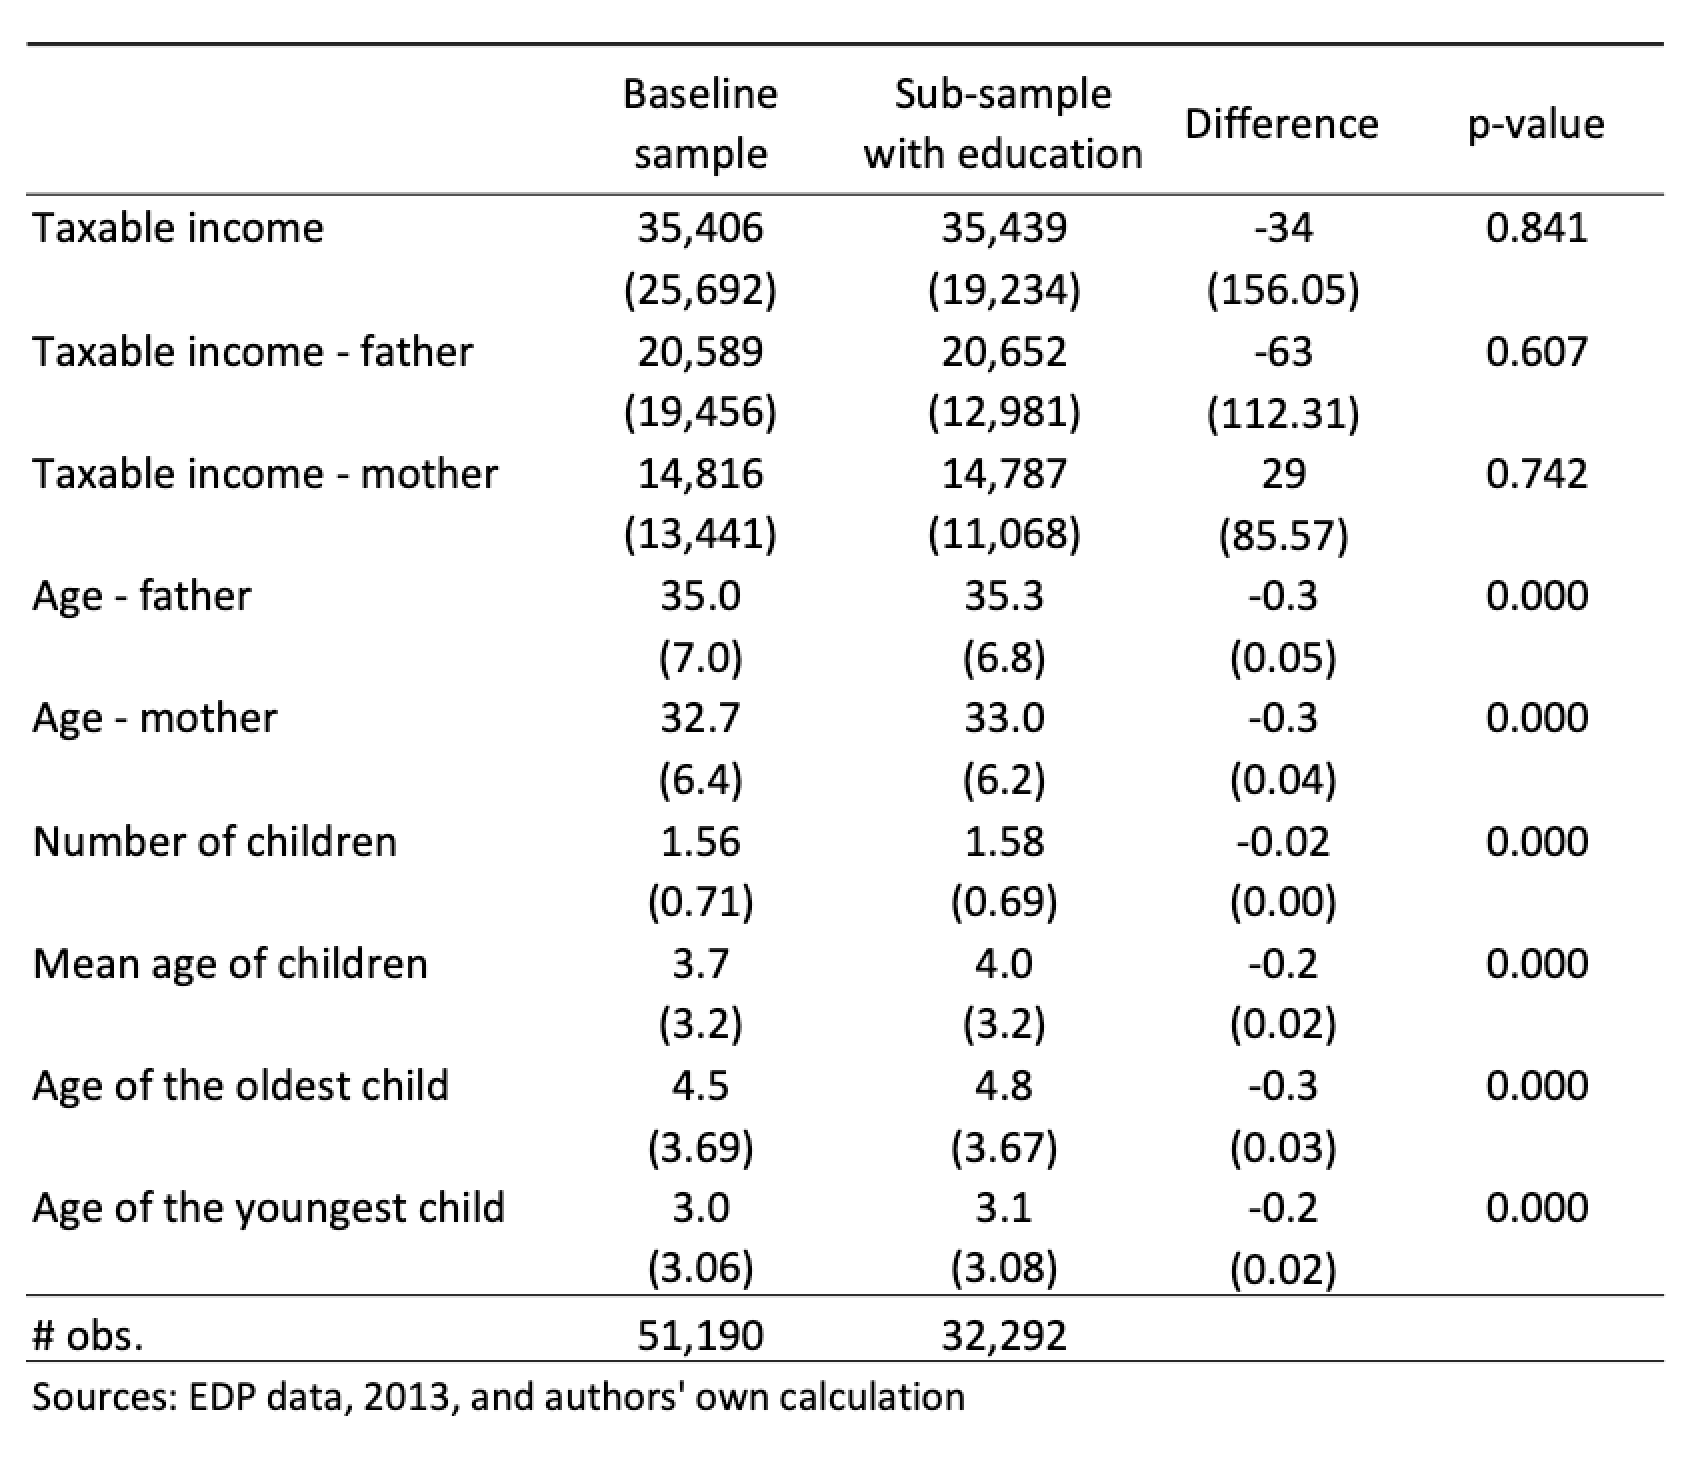
\includegraphics[width=1.1\textwidth]{figures/table_A_2.png}}%
    \label{tab:A2}

  \end{table}
\section{Marital Status Change and Large Non-Optimization}
  \begin{table}[H]
  \caption{\\Marital Status Change in 2014 and Large 
Non-Optimization in 2014:\\ Sensitivity Analysis
}
  \makebox[\textwidth][c]{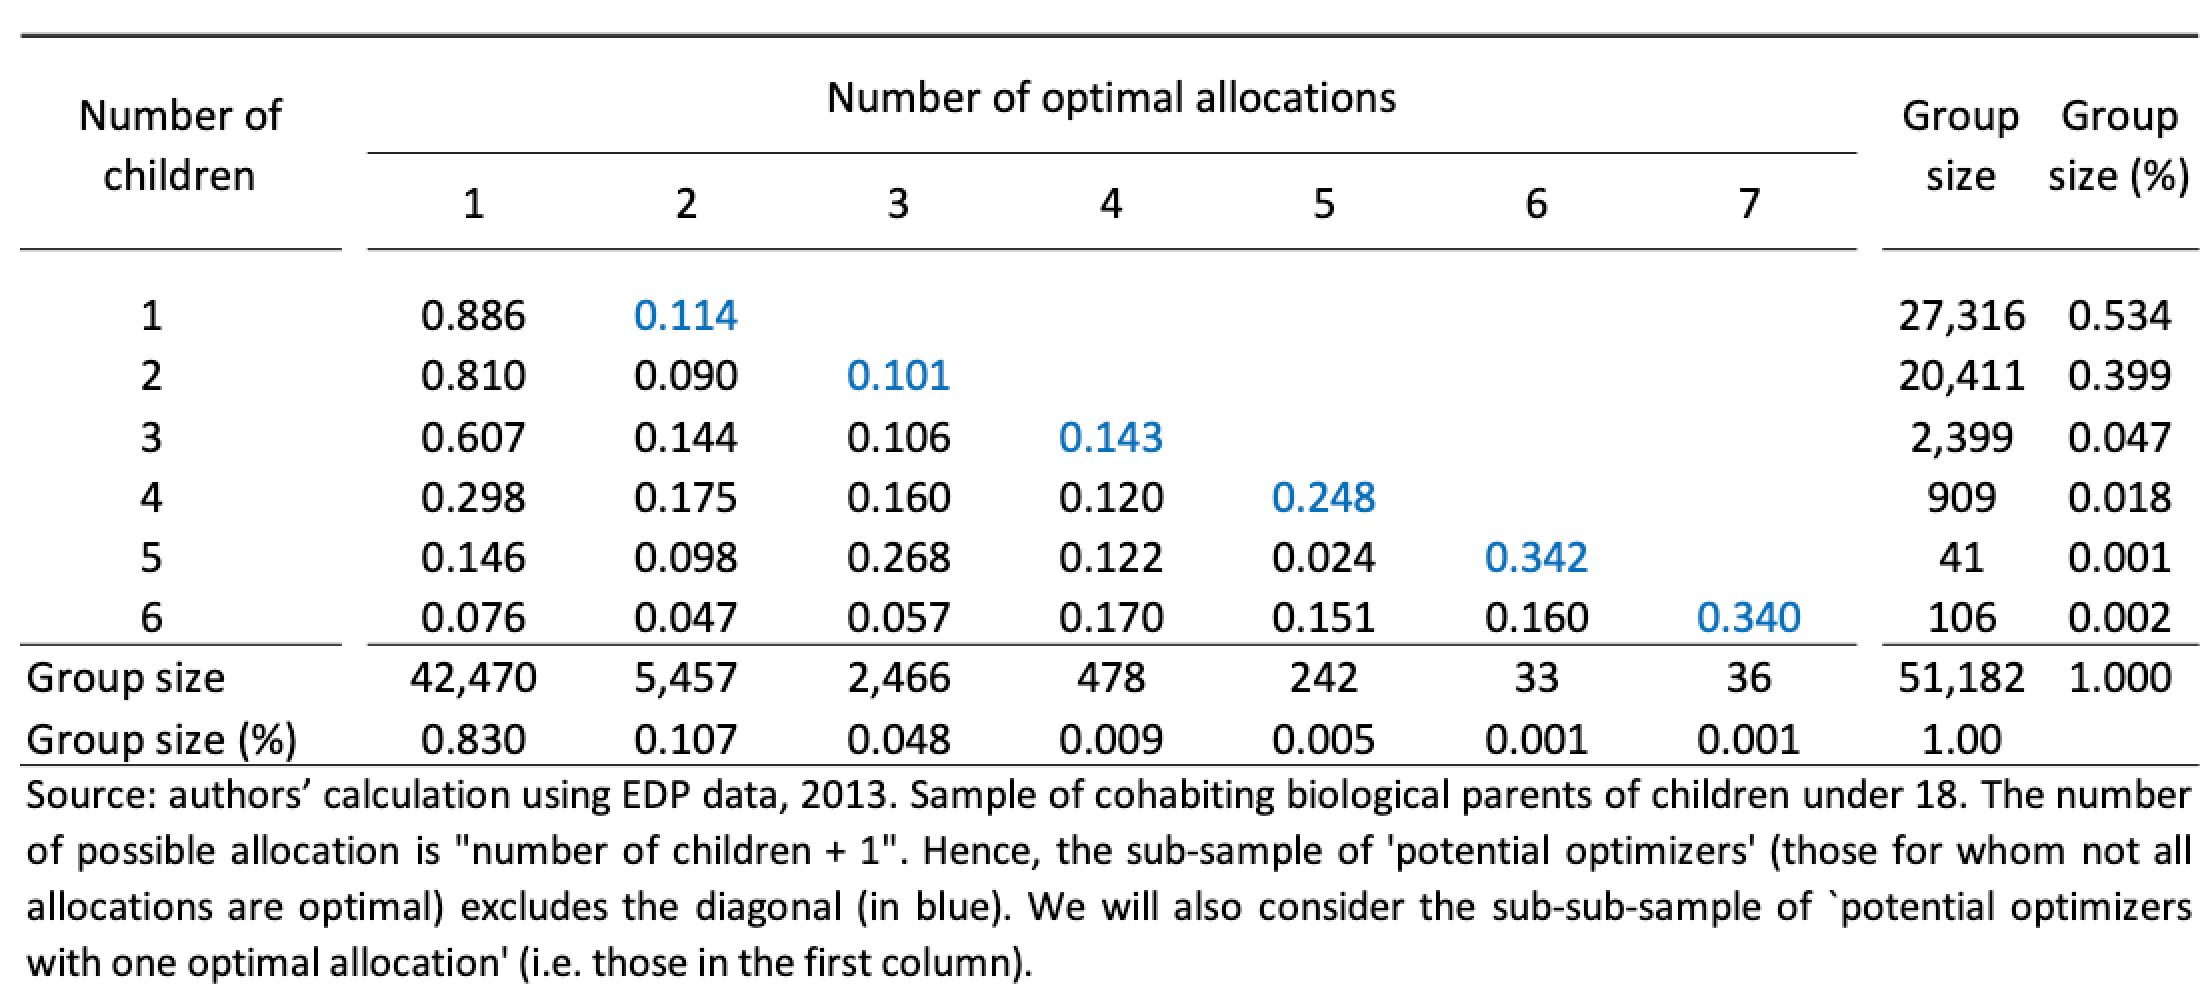
\includegraphics[width=1.1\textwidth]{figures/table_A_3.png}}%
  \label{tab:A3}
  \end{table}
\end{subappendices}
\ifx\isEmbedded\undefined
\newpage
%\bibliography{../Divers/biblio_these}
\end{document}
\else \fi